\chapter{ConTrib: Preventing Free-riding Behaviour with Decentralized Micro-accounting}
\label{chapter2}

\emph{We present \ModelName{}, a universal accounting mechanism to prevent abuse in shared-resource systems.
%In contrast to existing work, \ModelName{} does not make assumptions on the connected applications.
In \ModelName{}, each individual maintains a personal ledger with \emph{records}.
%A serialized micro-record with an empty payload is only 275 bytes and efficient to transfer.
Micro-records describe past interactions and link to other ones, resulting in a global, interconnected graph.
Fraud, specifically the forking of ones personal ledger, is detected by participants themselves through the exchange and validation of micro-records.
We devise a system architecture and implement it.
Our evaluation shows that forking of a personal ledger can be detected within a minute and with reasonable bandwidth overhead.
We also find that that the throughput of \ModelName{} scales linearly with the network size.
To explore \ModelName{} in a realistic environment, we deploy our mechanism in a Tor-like overlay and show how free-riders are detected.
This trial has resulted in over 125 million micro-records, created by more than \TrialUsers{} users.}

\newpage

\section{Introduction}

During the last decades, \enquote{Big Tech} companies have obtained significant market dominance in the information technology industry~\cite{frost2019bigtech}.
Companies such as Google, Amazon, Facebook, and Apple are omnipresent in our current society and even have the means of acting as small states, inhabited by billions of users worldwide.
By continuously broadening their activities, these companies seek to expand their virtual territory and seek to obtain monopolistic control over enabling elements for digital services, such as access to the Internet~\cite{best2014internet}.

The societal impact of \enquote{Big Tech} companies is a double-edged sword.
On the one hand, these companies are facilitating new modes of digital interaction between users, and also give rise to new business models.
The sharing economy is a prime example of this phenomena.
It is made up by digital markets for the trustworthy exchange of personal resources, such as houses and cars, between strangers~\cite{schor2016debating}.
This exchange process is a concept that has long been confined to trusted individuals, such as family and friends~\cite{frenken2019putting}.
Likewise, media platforms such as YouTube provide the required infrastructure for new forms of user engagement through video weblogging or \enquote{vlogging}.

On the other hand, it has become apparent that \enquote{Big Tech} companies tend to exploit their established market position and are increasingly involved in regulatory or political battles.
This behaviour sometimes goes undetected for years.
For example, researchers have only recently demonstrated that Uber actively manipulates the matchmaking process between passengers and drivers for commercial interests, therefore decreasing platform fairness and income equality of drivers~\cite{bokanyi2019ride}.
Similarly, Apple is currently under antitrust investigation by the European Commission that is assessing whether Apples' rules for developers on the distribution of apps via the App Store violate competition rules~\cite{kotapati2020antitrust}.

These concerning developments have contributed to increased efforts around the deployment of \emph{decentralized} applications that avoid centralized ownership.
Decentralized applications delegate the decision making away from a single authority.
A decentralized application mainly operates through the direct cooperation and information exchange between users, which we call \emph{peers}.
Arguably, Bitcoin is the most influential solution in this direction and provides a decentralized cash system without the supervision by an authoritative bank~\cite{nakamoto2019bitcoin}.
The underlying data structure of Bitcoin, a blockchain, is at the core of numerous decentralized applications~\cite{bashir2018mastering}.
At the time of writing, there are thousands of decentralized applications deployed on the Ethereum blockchain alone~\cite{wood2014ethereum}.
These decentralized applications include marketplaces, auctions, voting systems, lotteries, and games.

In contrast to the applications deployed by a company, decentralized applications are fully maintained by peers, without or with minimal involvement of a third party.
Decentralized applications require peers to pool their computer resources to provide the desired services to participants.
Specifically, peers have to communicate with other peers over the Internet, have to dedicate some computational power to process incoming messages, and frequently have to persist data.
Some decentralized applications critically depend on the voluntary contribution of computer resources by peers.
Bitcoin, for example, prevents the uncontrolled minting of digital coins through a resource-based consensus mechanism executed by miners~\cite{nakamoto2019bitcoin}.
These miners continuously solve a computational puzzle, a resource-intensive task that is required to the system secure.
Likewise, the Tor network provides anonymity by routing Internet traffic through volunteered relay and exit nodes~\cite{dingledine2004tor}.

Unfortunately, cooperation between peers in decentralized applications is hard to maintain.
Failing to reward peers for performing work can result in an unfair situation where peers can enjoy the services provided by other peers without reciprocating for longer times.
This detrimental behaviour, also called \emph{free-riding}, can degrade network performance in the long term, as dedicated peers will notice that their work is in vain and will ultimately leave~\cite{locher2006free}.
Measurements have demonstrated that free-riding often prevails in cooperative networks such as BitTorrent and Tor~\cite{sirivianos2007free}.
Since the cooperation between peers is at the heart of decentralized technology, we argue that this notion of fairness is a crucial requirement for \emph{any} decentralized application to ensure long-term sustainability~\cite{jelasity2004detection}.
With the renewed interest in decentralized alternatives for \enquote{Big Tech}, inducing fairness in decentralized applications is a significant challenge.
%Blockchain technology addresses this issue by requiring peers to pay a transaction fee when issuing transactions.
%Yet, the detection of abuse is non-trivial since the relevant data might not be immediately available. % is dispersed across the network.
%However, the deployment of decentralized platforms poses new technical challenges that have to be addressed.
%These challenges include identity management, data availability, inducing cooperative behaviour amongst peers, and abuse management.

%Since an operator has access to all historical events in a centralized system, detecting and addressing the abuse of resources is straightforward to achieve.
%This is more challenging in decentralized systems since information is dispersed across the network.

%\todo{bash centralized gatekeepers + antitrust}
%As a counterforce to the centralized architectures deployed by big tech companies, there has been significant effort to deploy decentralized systems that avoid third-party supervision.
%Blockchain technology, for example, empowers participants with a distributed ledger to securely record interactions and has been a key enabler of numerous decentralized systems like Bitcoin and Ethereum.
%Whereas the deployment of centralized systems is relatively straightforward, decentralized systems usually require additional complexity to mitigate the threats commonly found in decentralized networks.
%Significant research challenges include data availability and trust management.
%These threats include data unavailability, free-riding, and the Sybil Attack.

%\todo{alternative solution -> most feasible one is decentralized}
%\todo{prevent abuse in decentralized systems}

%At the heart of many systems, both centralized and decentralized, lies a mechanism for the secure storage and management of user-generated data.
%The storage and management of information in a decentralized system is a long-standing research challenge.
%Centralized service providers like Facebook and Amazon store all user data is stored on one or multiple servers that are fully under the control of the platform operator.
%On the other hand, secure and robust data management is considerably more challenging in decentralized networks where data must be stored by other, possibly untrusted peers.

%, with varying degrees of adoption.
%Perhaps the most influential example is Bitcoin, a digital currency that is fully maintained by its participating users.
%Bitcoin has demonstrated that it is possible to build a coin without banks.
%The core technology of Bitcoin, the distributed blockchain ledger, has bootstrapped much interest in decentralized alternatives.\todo{for example?}
%Another example is BitTorrent, a decentralized file-sharing protocol that enables users to directly exchange information.



%One might leverage blockchain technology to decentralized information management.
%Blockchain enables the tamper-proof and irrefutable storage of generic data elements, usually represented as transactions.

%Many of these innovations are pioneered by blockchain technology, which has been hailed as a panacea to disrupt these developments.
%Specifically, blockchain technology empowers users themselves to take on critical roles that are traditionally fulfilled by trusted authorities, e.g., banks, reshaping the notion of interactions in our society.
%Despite thriving ecosystems and markets worth billions of dollars (e.g., Ethereum), the first use case to pose a real threat to big tech companies has yet to be.
%This lack is mainly addressed to scalability limitations: blockchain technology is not performant enough yet to capture financial transactions on a global scale.

% The key challenge is to build a fully decentralized system, fully maintained by individuals. Requires adequate fraud prevention + free-riding prevention.

% One paragraph explaining how accounting in big-tech alternatives is different from existing work (e.g., PeerReview, Lifting, ...)

\begin{figure}[t]
	\centering
	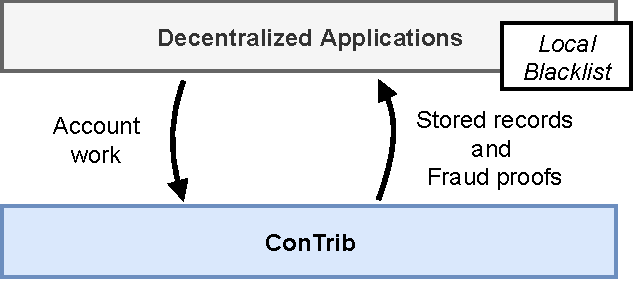
\includegraphics[width=.7\linewidth]{trustchain/assets/contrib_app_interaction}
	\caption{Decentralized applications can use \ModelName{} to account the work performed by peers within tamper-evident \emph{records}. These records are used by connected applications to detect free-riders and fraudsters, which are added to a blacklist. Applications can then choose to refuse services to the peers on the blacklist.}
	\label{fig:interaction_with_apps}
\end{figure}

% Argue about fairness?
% https://pdf.sciencedirectassets.com/272436/1-s2.0-S1084804516X00185/1-s2.0-S1084804516302788/main.pdf

\textbf{Our Solution.}
We induce fairness in decentralized applications by storing the description of work performed by peers in a distributed data structure.
Our universal mechanism, named \ModelName{}, is capable of accounting performed work within different decentralized applications.
With \ModelName{}, each peer maintains a \emph{personal ledger} with tamper-evident \emph{records}.
Records are created between two peers and describe some work performed by a peer for another peer, e.g., data exchange or file storage.
The design of \ModelName{} is lightweight and straightforward, yet enables the quick detection of \emph{fraud} targeted at the data structure.
This fraud occurs when a malicious peer forks its personal ledger and operates multiple versions of it in secret.
Peers continuously request random records from other peers and disseminate newly created records in the network.
To detect fraud, peers verify the consistency of incoming records with the ones in their local storage.

\ModelName{} enables connected applications to select which information should be recorded.
Figure~\ref{fig:interaction_with_apps} shows how a decentralized application can leverage \ModelName{} by accounting work, and by requesting records in the network to gather evidence of free-riding behaviour.
Each application maintains a blacklist with both free-riders and peers that have committed fraud by manipulating records.
Peers refrain from performing work for peers on the blacklist.
\ModelName{} is built to alleviate fairness concerns in a wide range of decentralized applications, including peer-assisted video distribution, anonymous communication networks, and distributed learning environments.
%Since \ModelName{} is agnostic about the application layer, different decentralized solutions can leverage \ModelName{} to securely record resource contributions and consumptions.

We implement \ModelName{} and evaluate different parameters that affect the efficiency of fraud detection, and on the communication overhead.
As we will demonstrate, fraud can be detected within a minute on average, even in networks with 10'000 malicious peers and under a conservative strategy for record exchange.
We also show that \ModelName{} highly tolerates packet loss and transient network failures.

To show the effectiveness of \ModelName{} in a realistic environment, we employ our accounting mechanism to address free-riding behaviour in \Tribler{}, a decentralized application downloaded by over 1.7 million users~\cite{pouwelse2008tribler}.
We use \ModelName{} to account bandwidth exchanges in \Tribler{}s' Tor-like overlay and use the accounted information to refuse services to free-riders.
Our two-year measurements have resulted in over \TrialRecords{} records, created by more than \TrialUsers{} users.
This large-scale deployment trial is a milestone in our ongoing research effort to solve the tragedy-of-the-commons in self-organizing Internet communities~\cite{de2018blockchain}.

The main contribution of this work is four-fold:
\begin{enumerate}
	\item \ModelName{}, a \emph{universal mechanism} that induces fairness in decentralized application by accounting work (Section~\ref{sec:micro_accounting} and \ref{sec:detecting_fraud}).
	\item A \emph{system architecture} around \ModelName{} with application-provided policies for record validation (Section~\ref{sec:system_architecture}).
	\item An \emph{implementation} and \emph{evaluation} of \ModelName{} with up to 10'000 peers, revealing the scalability of our mechanism and showing that fraud is detected within a minute on average (Section~\ref{sec:implementation_evaluation}).
	\item A \emph{large-scale deployment trial} of \ModelName{} in \Tribler{}, involving \TrialUsers{} Internet-recruited volunteers. This trial successfully addresses free-riding behaviour in \Tribler{} (Section~\ref{sec:deployment}).
\end{enumerate}

% We introduce ...

% Collective memory ...

%\section{Introduction}
%Free-riding, the act of selfishly benefiting from the usage of shared resources, is a common issue in both real-world and Internet communities~\cite{rose2003internet,adar2000free}.
%This selfish behaviour frequently prevails in Internet communities.
%This behaviour occurs when access to a shared resource is cheap and there are no individual consequences of overusing the good by community members.
%Structural free-riding on collective resources may result in a \emph{tragedy-of-the-commons}, the situation in shared-resource systems where the resource is depleted and the community around the resource collapses~\cite{hardin2009tragedy}.
%In this work, we address this behaviour by introduce a mechanism for digital shared-resource systems where all resource contributions and consumptions are accounted.
%Free-riding is a prevalent strategy within Internet communities.
%For example, digital media is aggressively competing for user attention, a scarce resource, through the unsolicited presentation of invasive banner ads and clickbait articles~\cite{chen2015misleading}.
%Ongoing Denial-of-Service (DOS) attacks on specific machines is another example of free-riding and shows that some individuals selfishly exploit the ubiquitous access to the Internet~\cite{cerf2013revisiting}.
%This behaviour shows that these attackers have a stronger incentive to undermine the security of shared Internet resources, rather than contributing to it.

%Shared-resource systems on the Internet are vulnerable to free-riding behaviour~\cite{locher2006free}.
%These systems are managing individuals with mutual access to computer resources offered to the community (e.g., bandwidth or CPU capacity).
%For example, downloading in the BitTorrent file-sharing network without contributing (seeding) back after the download has finished goes mostly unpunished and is therefore a common strategy~\cite{locher2006free}.
%Free-riding also occurs in anonymous networks like Tor, where users free-ride on the services offered by relay and exit nodes, without offering community services in return.
%Failure to acknowledge the presence of free-riding behaviour in peer-to-peer networks degrades the systems performance and could eventually result in users permanently leaving the network, as illustrated by the Gnutella software~\cite{adar2000free}.

%To date, the \emph{tragedy-of-the-commons} in Internet communities remains unsolved~\cite{harris2018institutional}.
%This social dilemma occurs where the community around a shared resource, e.g., storage capacity or bandwidth, will eventually collapse due to overexploitation when individual self-interest is at odds with community interests.
%A well-known example is \emph{free-riding} in file-sharing networks, where the act of downloading content without contributing (seeding) back after the download has finished goes mostly unpunished~\cite{locher2006free}.
%Long-term non-cooperative behaviour in shared-resource systems degrades the network performance and eventually leads to a community collapse as illustrated by peer-to-peer applications like  Gnutella~\cite{adar2000free}.

%The Internet has turned into a grim place, where selfish interest of big tech companies supersedes the importance of user-managed communities.
%Email spam is a prominent example of what happens when bandwidth is abused for selfish reasons.
%Over 45\% of email traffic consists of junk messages and an increasing number of ISPs and hosting providers are being forced to use sophisticated techniques in order to try at least to reduce it.
%Likewise, digital media is competing for user attention through the unsolicited presentation of invasive banner ads and clickbait articles.
%Ongoing DDoS attacks on specific machines show that some individuals have a stronger incentive to undermine the security of the Internet, rather than contributing to it.



%Oftentimes, the allocation of shared resources such as bandwidth is prescribed by the output of an algorithm that considers all historical contributions and consumptions of a peer~\cite{tang2004trust}.
%This trust can be based on historical action, or on a believe that the other agent will reciprocate a service later.
%Trade-based incentive mechanisms rely on remuneration for the volunteer resource sharing by agents, either through credits or monetary value.
%This is the approach taken by volunteer computing services, e.g., Boinc, and blockchain-based resource markets, e.g., FileCoin~\cite{benet2018filecoin} and Orchid~\cite{cannellorchid}.

%Providing meaningful incentives to reciprocate after taking some of its resources is imperative to alleviate free-riding behaviour and boost cooperating amongst participants~\cite{ma2004incentive}.
%Some shared-resource systems rely on a \emph{trade-based incentives} where resource consumption is immediately remunerated using a credit or payment system.
%For example, in many volunteer computing projects offered by BOINC users are rewarded for their contributed resources with virtual credits.
%Likewise, shared-resource systems build on blockchain technology leverage cryptocurrency payments to reward communal services~\cite{benet2018filecoin}.

%With \emph{trust-based incentives}, community members are indirectly reciprocated.
%Usually, the amount of provided and consumed resources to and from the community is expressed in a trust score, which can be computed by a reputation mechanism~\cite{meulpolder2009bartercast}.
%These scores are then used to determine a fair allocation of resources, for example, peers with a higher reputation are granted preferential treatment during periods of congestion.
%These trustworthiness scores can be computed by a reputation algorithm.
%To accurately determine the trustworthiness of individuals, shared-resource systems require a public accounting mechanism that records all interactions between users.
%This work focusses on secure accounting of interactions in such systems.

%There have been several proposals to address free-riding behaviour by securely accounting interactions~\cite{guerraoui2010lifting,haeberlen2007peerreview,mokhtar2014acting}.
%We find, however, that existing work is lacking in two directions.
%First, the design of existing solutions usually considers a specific application, e.g., file-sharing or gossip networks.
%This makes it hard, if not impossible, to re-use these solutions across shared-resource systems with differing resource types.
%Second, existing solutions tend to elevate the authority of specific peers in the network, e.g., by having a user act as witness for others.
%This introduces additional system complexities, e.g., incentivize users to not abuse their authority and to follow the protocol.

%As research points out, the interactions in digital shared-resource systems are usually short-lived and concern a small amount of resources~\cite{seuken2014work}.
%For example, the storage protocol FileCoin~\cite{benet2018filecoin} splits data into many small pieces and remunerate peers for the retrieval of individual pieces.
%Similarly, the BitTorrent file-sharing protocol orients around the transport of small data pieces with a variety of peers.
%Repeated, small interactions allows for lower risk-taking since peers can abort an interaction when its counterparty defects, e.g., when a counterparty goes offline during a file exchange.


%This approach aligns well with existing shared-resource systems where interactions are short-lived and concern a small amount of resources~\cite{seuken2014work}.
%For example, blockchain-based storage networks like FileCoin~\cite{benet2018filecoin} split data into small pieces and remunerate peers for the retrieval of pieces.
%Furthermore, micro-accounting allows for low risk-taking since peers can abort an interaction when its counterparty defects, e.g., when a counterparty goes offline during a file exchange.


%In this work, we design, implement, deploy and evaluate a 
%We identify two key advantages of micro-accounting

%So far, there is no lightweight and reusable \emph{micro-accounting} mechanism, specifically designed for recording small interactions in large shared-resource systems.

%Currently, there is no lightweight mechanism for tamper-proof accounting of community interactions, to the best knowledge of the authors.

% Motivate the need for micro-accounting
% 1) it aligns well with existing systems, e.g., file sharing and bandwidth sharing
% 2) it allows for quick punishment and blacklisting of users, with low value-at-risk

%So far, there has been a wide range of research in designing incentive-compatible mechanisms to prevent free-riding in decentralized networks.
%Many of the proposed models and mechanisms require secure accounting of community contributions, for example, if a peer has donated some storage to a specific peer or has uploaded a file to others.

%Most of these efforts are concentrated on reducing free-riding behaviour in file-sharing communities.
%However, free-riding is also prevalent in other communities, such as anonymity networks~\cite{biryukov2015proof}.
%We also observe that most research in this direction take a clean-slate approach for the implementation of their mechanisms.
%This leads to a large range of different implementations.
%Specifically, there is no universal, resource-agnostic infrastructure to quickly evaluate new mechanisms and policies.
%We argue that furthefr research on the management of Internet commons benefits from such an infrastructure.
%Many of these solutions share commonalities in the infrastructure required to deploy these mechanisms.

%\begin{figure}[b]
%	\centering
%	\includegraphics[width=\linewidth]{assets/components}
%	\caption{Our model for trust-based management of shared Internet resources such as bandwidth and storage.}
%	\label{fig:model}
%\end{figure}

%\begin{figure}[t]
%	\centering
%	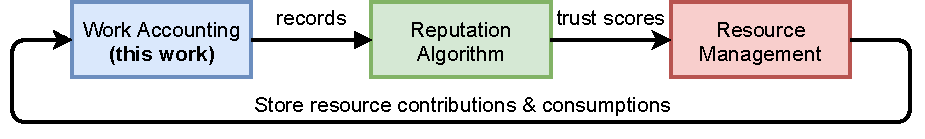
\includegraphics[width=\linewidth]{assets/trust_cycle}
%	\caption{Our envisioned approach to address free-riding behaviour in large-scale shared-resource systems.}
%	\label{fig:trust_cycle}
%\end{figure}

%We present \ModelName{}, a universal accounting mechanism for the detection of free-riding behaviour in shared-resource systems.
%Our mechanism enables resource accounting where fraud, e.g., illegitimate tempering of micro-records, can be efficiently detected across different shared-resource applications.
%\emph{Micro-records} are the key building block of \ModelName{} and are linked together in a personal ledger.
%A micro-record describes an interaction from the perspective of one of the involved parties.
%Users continuously share micro-records with random users and validate incoming micro-records against known ones.
%Our simple, yet effective technique enables quick detection of fraud, specifically the situation where an adversary has forked its personal ledger.
%We implement \ModelName{} and systematically evaluate its scalability and resistance against malicious users that undermine the accounting mechanism, e.g., by hiding or modifying the micro-records in their personal ledger.
%Our experiments with up to 1'000 users reveal that \ModelName{} that fraud can be detected well within a minute and that the throughput of \ModelName{} scales linearly with the network size.

%To show the effectiveness and matureness of \ModelName{} in a realistic environment, we leverage our mechanism to record bandwidth traffic in \Tribler{}.
%\Tribler{} is our academic peer-to-peer software and downloaded by over 1 million users.
%Specifically, we use \ModelName{} to account bandwidth exchanges in our Tor-like overlay and refuse services to free-riders during periods of congestion.
%Our 36-months measurements has resulted in over 120 million micro-records, created by over \TrialUsers{} users.
%This large-scale deployment trial is a key milestone in our ongoing research to solve the tragedy-of-the-commons in Internet communities.

%The \ModelName{} mechanism is based on two principles.
%First, we decouple the application logic and accounting primitives, unlike related work in the same domain~\cite{osipkov2006robust}.
%This results in a universal accounting mechanism that is reusable across different application domains.
%Second, \ModelName{} is specifically built to deal with the dynamic nature of peer-to-peer networks, where users quickly join or leave.
%Specifically, we avoid network-wide synchronization, group communication or the explicit management of witness sets, while ensuring that fraud will be detected with reasonable probability.

%This work is a cardinal part of our envisioned approach to solve the tragedy-of-the-commons, see Figure~\ref{fig:trust_cycle}.
%In this approach, peers account all resource contribution and consumptions within tamper-proof \emph{micro-records}.
%\ModelName{} records resource contributions and consumptions.
%Our envisioned next step is that every community member periodically runs a reputation algorithm on the collected micro-records which outputs subjective trustworthiness scores.
%These scores guide resource management, the process of determining which users will be granted access to some shared resource.

%Micro-records are organized in personal ledgers and can capture bilateral interactions between individuals by pointing to other micro-records.

%We identify the components and policies that together form an infrastructure for trust-based management of Internet resources.
%Our middleware is flexible, unlike blockchain-based approaches that require full replication and network-wide consensus.
%We build our middleware based on the model visualized in Figure~\ref{fig:model}.
%All community contributions are recorded on a light-weight and tamper-proof distributed ledger and used to compute trust scores by agents.
%These trust scores are then used to allocate resources to others.
%We identify, design and implement the required policies for the management of Internet resources in decentralized communities.

%We believe that the tragedy of the Internet commons can be solved through trust-based mechanisms.
%In this work, we build the required digital infrastructure and tools for sustainable community management on the Internet: accounting mechanisms, reputation algorithms, allocation policies.
%All presented components have been evaluated and tested through field trials with real users, using our academic software named Tribler.
%Tribler is the result of 15 years of engineering effort and has been downloaded by over 1.x million users.

% Possible system attacks:
% Free-riding
% Misreporting
% Collusion
% White-washing

\section{Background and Problem Description}
The challenge at hand is to address free-riding behaviour and induce fairness in decentralized applications.
Many solutions reward peers for performing work in the system~\cite{ma2004incentive}.
We first outline two existing approaches to incentivize the cooperation of peers, namely trade-based and trust-based incentives~\cite{ruffo2007fairpeers}.
Finally, we describe the requirements for our solution and elaborate on accompanying challenges.

\subsection{Trade-based Approaches}
With trade-based approaches, performed work by peers is remunerated using a credit or payment system.
This remuneration either occurs immediately after the work is performed, or a peer performs payments in batches.
The main idea is to rewarded work with credits, whereas peers that use the services of other peers are required to pay.
The accrued credits can either be converted to real-world money or are merely useful to show the dedication of a particular peer.
BOINC is a well-known volunteer computing project rewards users for their computational power with virtual credits~\cite{anderson2019boinc}.

Blockchain technology relies on financial remuneration to keep the system secure~\cite{easley2019mining}.
Miners, dedicated peers that invest computational power to maintain the blockchain ledger, are usually rewarded for their efforts by the system and by users that issue new transactions.
Users pay fees to get their transaction included in the distributed ledger.
Miners then collect these fees when including transactions in the blockchain.
Some decentralized applications have adopted cryptocurrencies as a payment system to reward performed work.
Filecoin is a decentralized system where users pay a fee to have their data stored by peers~\cite{benet2018filecoin}.
Likewise, TorCoin proposes a mechanism where the relay and exit nodes \enquote{mine} a Bitcoin-derived cryptocurrency by relaying Internet traffic~\cite{ghosh2014torpath}.

Even though trade-based incentives are frequently used to incentivize work, remuneration techniques are not an adequate solution for any decentralized applications, for the following two reasons~\cite{hummel2003earning}.
First, they require the integration of a secure payment infrastructure which complicates the system design and potentially enables new forms of attack, such as coin forgery and double-spending.
If a central authority is used to keep track of each peer's balance, there now is a single-point-of-failure.
Second, remuneration can result in new forms of unfairness where a few rich peers exclusively enjoy the services of a decentralized application.
This situation could arise, for example, when operating peer-to-peer auctions for the allocation of services.

\subsection{Trust-based Approaches}
With trust-based approaches, community members are indirectly reciprocated for their work, for example, by getting preferential treatment.
This often involves peers keeping track of the long-term contributions of each peer.
This requires infrastructure to account all performed work by peers~\cite{meulpolder2009bartercast}.
The details of accounted work can then be used by the application to detect if a specific peer is free-riding.
In practice, the accounted work is usually fed into a reputation algorithm that outputs a ranking~\cite{karakaya2009free}.
If the ranking of a specific peer is low, the application can decide to refuse serving this peer until its ranking has improved.
%Blockchain technology also provides accounting capabilities and empowers users with a distributed ledger to securely store their interactions~\cite{underwood2016blockchain}.
%However, we consider blockchain unsuitable for accounting purposes since maintaining the distributed ledger is prohibitively expensive.\todo{defend this statement}

Wallach et al., present different mechanisms for the fair sharing of resources in decentralized applications through the usage of log inspections and random auditing~\cite{wallach2003enforcing}.
Their work, however, exclusively focusses on storage-based systems.
To the best of our knowledge, their design is not reusable for other decentralized applications, limiting the applicability of their work.
Similarly, the work of Osipkov et al., describe an accounting mechanism for file-sharing networks where each peer maintains a set of witnesses that monitors all transactions of that peer~\cite{osipkov2006robust}.

LiFTinG and AcTinG are protocols for tracking free-riding behaviour in gossip-based systems~\cite{guerraoui2010lifting,mokhtar2014acting}.
The LiFTinG protocol exploits the message dynamics between peers, e.g., that the content received by a peer is further propagated according to the protocol.
The design depends on a statistical approach and cross-checking of logs to detect free-riders but is not reusable for applications beyond gossip.

Another approach is to maintain a distributed ledger that tracks the work in decentralized applications.
%Vegvisir is a partition-tolerant blockchain that leverages conflict-free replicated data types (CRDTs) to build a direct acyclic graph with transactions~\cite{karlsson2018vegvisir}.
PeerReview is an accountability mechanism to record message exchange between peers~\cite{haeberlen2007peerreview}.
Peers store all network messages in a local log.
Dedicated witnesses continuously audit peers and detect whether a peer deviates from the protocol.
The FullReview protocol extends PeerReview by addressing selfish behaviour with a game-theoretical model~\cite{diarra2014fullreview}.
%Their work also describes an experiment that shows how free-riding behaviour in multicast can be detected.
Otte et al., present TrustChain, a Sybil-resistant reputation mechanism with an accompanying accounting mechanism~\cite{otte2017trustchain}.
The authors apply their mechanism to address free-riding behaviour in a file-sharing network.
We find that peers in TrustChain cannot engage in the recording of multiple interactions simultaneously, significantly limiting the achievable throughput.
Crosby et al., presents a data structure for tamper-evident logging~\cite{crosby2009efficient}.
This data structure is primarily focussed on the logging of unilateral system events on a server.

\subsection{Problem Description}
\label{sec:problem_description}
There currently is no \emph{universal} accounting mechanism that is capable of addressing free-riding behaviour and improve fairness in decentralized applications.
We address this shortcoming and describe three challenges when designing such a mechanism.

\textbf{Challenge I: Universality.}
The accounting solutions that we have identified so far are built for a single application type and are infeasible to re-use across different domains.
We believe that universality is an important requirement to address fairness concerns in decentralized applications.

\textbf{Challenge II: Avoid Central Authorities.}
To keep our system reusable and generic, we avoid \emph{any} decision making by entities with leveraged authorities and central servers.
The lack of a central authority makes our mechanism \emph{fully decentralized}.
In general, decentralized mechanisms are less vulnerable to large-scale attacks, tend to scale better, and are more resilient to failure.
They also are an excellent architectural fit with existing decentralized applications without central authorities.

\textbf{Challenge III: Fraud Detection.}
When accounting work in a decentralized application, peers will have a natural incentive to misrepresent the magnitude of their efforts to inflate their social standing, or to hide information unfavourable to their standing~\cite{meulpolder2009bartercast}.
Our accounting mechanism must address the completeness and correctness of the stored information.
We must \emph{detect the manipulation or hiding of accounted information} and punish adversarial peers accordingly.
%Since different applications are likely to have differing visions on how fraud should be managed, we leave this decision to the application.

%For example, overuse in a file-sharing system can result in a temporary, e.g., 24-hour, ban or even result in ostracization from the community.

%\textbf{Requirement III: Scalability.}
%Open shared-resource systems on the Internet can grow to moderate or large sizes.
%For example, applications like BitTorrent and Tor are used by millions of users.
%We require that our solution \emph{scales} when the network size and number of interactions grow.

%Blockchain technology is increasingly being used to manage shared-resource systems.
%FileCoin, for example, is a decentralized system for renting out user-volunteered storage~\cite{benet2018filecoin}.
%Participants in FileCoin record all interactions (data exchanges) within transactions on a distributed ledger, fully maintained by participants.
%Transactions are bundled in blocks, and each block contains the hash of the prior block.
%The modification of a transaction in one block is detected while reaching a distributed consensus.

%Despite a growing ecosystem around the deployment of blockchain-based applications, blockchain technology have fundamental scalability limitations.
%The key issue is that the network is required to continuously establish consensus on the entire transaction set~\cite{vukolic2015quest}.
%This consensus process is carried out by \emph{miners}, volunteers that manage the blockchain.
%The need for consensus significantly limits the achievable throughput, and imposes high storage and bandwidth requirements.
%The throughput of a blockchain secured by Proof-of-Work is usually limited to hundreds transactions per second at best, by far not sufficient to record interactions in large-scale shared-resource systems.
%Furthermore, participants are required to store the full blockchain, which can grow to considerable sizes (e.g., the Bitcoin blockchain currently requires around 290 GB of storage).\footnote{See https://www.blockchain.com/charts/blocks-size}
%We require a lightweight solution, suitable for deployment in large-scale networks.

%Scalability concerns are partially addressed by layer two solutions, e.g., state channels~\cite{mccorry2019pisa}.
%Transactions in layer two solutions are conducted off-chain and users maintain channels to route payment to other users. % users to create transactions 
%Yet, this technology still rely on a \enquote{primary} blockchain for channel management and dispute resolution.


%\textbf{Requirement III: Full decentralization.}
%Many shared-resource systems avert manipulation concerns by introducing a centralized manager that manages all credits or reputation scores of network participants (e.g., as in BOINC).
%However, users now have to trust the manager that it does not modify the credit or trust scores.
%Furthermore, a centralized manager complicates integration with existing systems since it introduces new roles and adds an additional dependency on external actors.
%In practice, dependency on a critical entity introduced a single point-of-failure since downtime of this entity stall all activity.

%As an alternative, one can leverage semi-decentralized solutions where a group of peers are charged with the system management.
%Blockchain is a semi-decentralized system since there is usually a group of peers of which the majority is assumed to be honest.
%Also, the PeerReview accounting mechanism uses witnesses to periodically inspect the correct behaviour of participants in the network~\cite{haeberlen2007peerreview}.

%This work specifically focusses on resource tracking in shared-resource systems.\todo{do something with this}
%There have been proposals to introduce accountability in distributed systems to either detect faulty behaviour or free-riding.

%Even though it is impossible to establish that the interaction embedded in a record has actually occurred, our micro-accounting mechanism should be able to handle record manipulation.

% Problem 1: detect manipulation
% Problem 2: avoid reliance on TTP

%\begin{figure*}[t!]
%	\centering
%	\begin{subfigure}[t]{.33\textwidth}
%		\centering
%		\captionsetup{width=.9\linewidth}
%		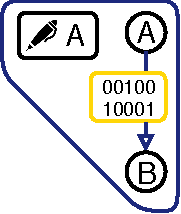
\includegraphics[width=.65\linewidth]{assets/tutorial_1}
%		\caption{To record an interaction between $ A $ and $ B $, $ A $ creates and sign a proposing micro-record (also called a \emph{proposal}).}
%		\label{fig:trustchain_tutorial_1}
%	\end{subfigure}%
%	\begin{subfigure}[t]{.33\textwidth}
%		\centering
%		\captionsetup{width=.89\linewidth}
%		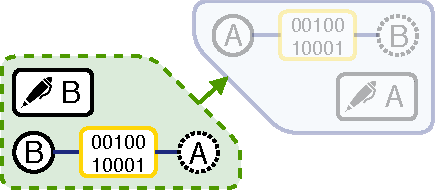
\includegraphics[width=.85\linewidth]{assets/tutorial_2}
%		\caption{Next, $ B $ confirms $ A $'s proposal by creating a confirming micro-record (also called a \emph{confirmation}), that points to it.}
%		\label{fig:trustchain_tutorial_2}
%	\end{subfigure}%
%	\begin{subfigure}[t]{.33\textwidth}
%		\centering
%		\captionsetup{width=.93\linewidth}
%		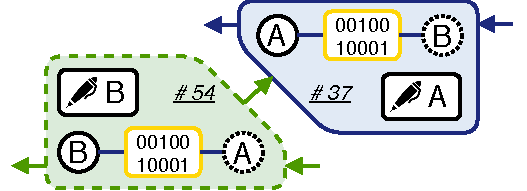
\includegraphics[width=.98\linewidth]{assets/tutorial_3}
%		\caption{To ensure tamper-proofness, we organize micro-records in personal ledgers and reference prior micro-records in a ledger.}
%		\label{fig:trustchain_tutorial_3}
%	\end{subfigure}
%	\caption{Storing an interaction between users $ A $ and $ B $ in \ModelName{} using two micro-records, one proposal and one confirmation. Solid and dotted circular elements indicate the identity of the micro-record creator, respectively, the micro-record counterparty.}
%	\label{fig:trustchain_tutorial}
%\end{figure*}

\section{Accounting Work with \ModelName{}}
\label{sec:micro_accounting}
The design of our accounting mechanism, named \ModelName{}, is inspired by the tamper-proof properties of blockchain ledgers, but does not require peers to reach agreement on a coherent history of records.
As such, inappropriate behaviour of a few peers does not result in system-wide failures.
In summary, \ModelName{} optimistically detects the illegitimate modification of records while keeping the computational requirements and bandwidth overhead low.
Decentralized applications account the work performed by peers within \emph{records}.
Each peer organizes their records in a \emph{personal ledger}.
A record describes some work performed by one peer for another peer.
Records point to prior records in the same personal ledger, and also to records in the personal ledger of others.
The latter pointer captures an agreement between two peers.
Peers continuously exchange records with other random peers.
By validating the consistency of incoming records against known ones, fraud can irrefutably be proven.
\ModelName{} enables the construction of an irrefutable fraud proof which can be shared with others.

We further elaborate on the design of \ModelName{}.
We first outline the network and threat model.
We then describe the \ModelName{} data structure and show how \ModelName{} accounts the work in decentralized applications.
%In \ModelName{}, an interaction indicates a small contribution or consumption of resources.
%The accounting of this interaction can proceed before or after the resources have been exchanged.

\subsection{Network Model}
\label{sec:network_model}
\ModelName{} builds on a peer-to-peer network.
We assume an unstructured network structure all peers maintain roughly the same number of connections with other peers.
Unstructured networks are relatively straightforward to maintain and highly resilient against churn.
Network bootstrapping and peer discovery functionality should be provided by the adopted network library.
We also assume that the communication channels between peers are unreliable and unordered (e.g., by using the UDP communication model).
The arrival time of messages is not upper bounded and outbound messages can fail to arrive at the intended destination.
Each peer is in possession of a cryptographic keypair, consisting of a public and private key.
The public key uniquely identify the peer whereas the private key is used to digitally sign records and outgoing network messages.
We consider attacks targeted at the network layer, e.g., the Eclipse Attack, outside the scope of this work.

A prominent threat in peer-to-peer applications is the Sybil Attack, where an adversary operates multiple identities to either inflate its own social standing or to subvert the network~\cite{douceur2002sybil}.
This is particularly important in open Internet communities, where the cost of creating a new digital identity is often negligible.
We consider the full implications of the Sybil Attack outside the scope of our work.
We believe, however, that self-sovereign identities are a promising avenue that can complement decentralized networks to address this threat~\cite{stokkink2018deployment}.

We also consider misreporting, the inaccurate recording of work that have not actually occurred in the system, beyond the scope of this work.
This is challenging to address in a generic way since there is not always a straightforward method to determine if some work has actually occurred in the system.
Some protocols leverage cryptographic techniques to prove the accuracy of performed work, e.g., Proof-of-Storage or Proof-of-Bandwidth~\cite{benet2018filecoin,ghosh2014torpath}.
These proofs, however, cannot be used beyond a specific application domain.
Misreporting can also detected and taken into consideration by the algorithm that processes the accounted work~\cite{seuken2010accounting}.

\subsection{Threat Model}
\label{sec:threat_model}
Our threat model orients around malicious peers that strategically manipulate their \ModelName{} records, either by sharing tampered records or by withholding specific records.
For example, a peer can try to inflate the amount of work it has performed in the past by changing one of its records.
In \ModelName{}, this attacks manifests by users operating on multiple copies of their personal ledger, possibly returning records from different ledger copies to distinct peers.
As discussed in Section~\ref{sec:problem_description}, we require that this malicious behaviour can be detected.
We assume that the compute power of adversaries is bounded and that cryptographic primitives are secure.

%A particular treat is when peers collude in order to record false information, e.g., a bandwidth upload that has not actually occurred within the system.
%It is non-trivial to verify whether the interaction has actually occurred in the system and therefore, we consider this attack outside our scope.
%Addressing this attack likely requires a mechanism that leverages application-specific properties.
%For example, TorPath builds a proof-of-bandwidth that proves that some bandwidth has been transferred through a circuit~\cite{ghosh2014torpath}.
%Creators of fake information should be given a lower trust score by the reputation mechanism, as illustrated in Figure~\ref{fig:trust_cycle}.

%Users store dual-signed agreements of their interactions using \ModelName{} in \emph{micro-records}.

%\begin{table}
%\begin{center}
%	\begin{tabular}{ | p{1cm} | p{6.5cm} | }
%		\hline
%		\textbf{Field} &\textbf{Description} \\
%		\hline
%		$ i $ & The index of the micro-record in the personal ledger of $ a $. \\
%		$ a_{pk} $ & The public key of $ a $. \\
%		$ b_{pk} $ & The public key of $ b $. \\
%		$ t $ & The type of the micro-record. \\
%		$ p $ & The payload of the micro-record. \\ 
%		$ s_{a,i} $ & A digital signature by $ a $ over the micro-record. \\ 
%		$ h_{a,i-1} $ & The hash of the previous micro-record in the personal ledger of $ A $. \\ \hline
%		$ l $ & The index of the referenced proposal. \\ 
%		$ h_{b,l} $ & The hash of a referenced proposal. \\
%		\hline
%	\end{tabular}
%\end{center}
%\caption{The fields in a micro-record created by user $ a $, capturing an interaction with user $ b $. A proposal does not contain the last two fields ($ l $ and $ h_{b,l} $).}
%\label{tab:micro_record}
%\end{table}

\begin{figure}[t]
	\centering
	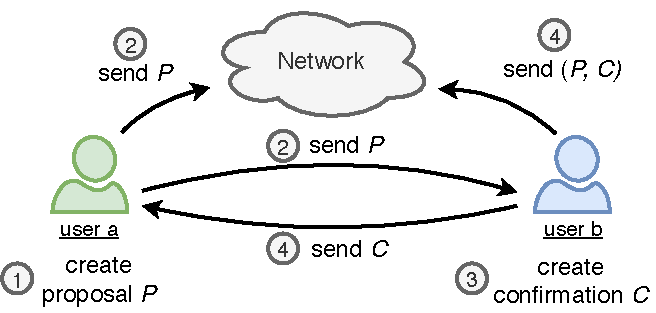
\includegraphics[width=.75\linewidth]{trustchain/assets/interaction}
	\caption{The process of recording work between peers $ a $ and $ b $ using two records: a proposal $ P $ and a confirmation $ C $.}
	\label{fig:interaction}
\end{figure}

\subsection{Recording Interactions}
\label{sec:recording_interactions}
\ModelName{} records performed work in \emph{records}.
A record describes some work performed by a particular peer for another peer.
%Each micro-record is either a \emph{proposal} or a \emph{confirmation}.
Some work that involves peers $ a $ and $ b $ is recorded using two records: one \emph{proposal} created by $ a $ and one \emph{confirmation} created by $ b $.
This process is visualized in Figure~\ref{fig:interaction}.
First, $ a $ creates a proposal record that records work involving $ b $ (step \circled{1}).
We refer to this proposal as $ P $.
We define proposal $ P $, created by peer $ a $, as a tuple with the following attributes:
\begin{align*}
	P = (\texttt{pubKey}, \texttt{pubKeyOther}, \texttt{payload}, \texttt{sig})
\end{align*}
$ P $ contains the public key of peers $ a $ and $ b $ (\texttt{pubKey} and \texttt{pubKeyOther}, respectively), an application-specific payload \texttt{payload}, and a digital signature \texttt{sig} by $ a $ over the record content in binary form.
We will use this notation when describing our fraud detection algorithms in Section~\ref{sec:detecting_fraud}.
The payload can be an arbitrary blob of data and is provided by the application.
To increase the resilience against manipulation, we extend records with additional fields later.
%A transaction is a generic description of any interaction between users, for instance, making an agreement or recording a trade.
%We consider a transaction to be the result of \emph{any} interaction between users, like transferring assets or recording agreements. %We intentionally consider a transaction to be a description of any interaction between two users.
% As a result, it can describe almost every interaction between two or more users, like asset transfers or generic agreements.
After $ a $ included all described fields in the proposal, the record is persisted to $ a $'s database, sent to $ b $, and disseminated to $ f $ random users in the peer-to-peer network (step \circled{2}).
We refer to $ f $ as the \emph{fanout} value.

%A micro-record created by user $ a $, capturing an interacting with $ b $ is defined as a tuple $ R_{a,i} = (i, a_{pk}, b_{pk}, t, p, s_{a,i}, h_{a,i-1}, l, h_{b,l}) $.
%All fields in $ R_{a,s} $ are listed and described in Table~\ref{tab:micro_record}.
%Every micro-record is equipped with a sequence number $ i \in \mathbb{Z} $ that indicates the index of the micro-record in the personal ledger of the creating user.
%It also contains the public keys of both interacting users.
%A micro-record created by $ a $ contains a hash pointer ($ h_{a,i-1} $) to the previous micro-record in the personal ledger of $ a $.

When $ b $ receives the proposal $ P $, $ b $ verifies its validity.
It is during this step that fraud is detected.
The validation logic of records is discussed later in this work, see in Section~\ref{sec:detecting_fraud}.
If the incoming proposal $ P $ is valid, $ b $ determines if the payload in $ P $ truthfully describes the performed work, according to the knowledge of $ b $.
If not, $ b $ ignores the incoming proposal and takes no further action.
Otherwise, $ b $ creates and signs a confirming record, denoted by $ C $, that confirms $ P $ (step \circled{3}).
This confirmation contains the same fields as the proposal $ P $ and also includes the hash of $ P $.
We define confirmation $ C $, created by peer $ b $, as the following tuple:
\begin{align*}
	C = (\texttt{pubKey}, \texttt{pubKeyOther}, \texttt{payload}, \texttt{proposalHash}, \texttt{sig})
\end{align*}

The value of \texttt{prevHash} is given by $ H(P) $, where $ H(\cdot) $ is a secure hash function.
We call the \texttt{prevHash} value in $ C $ the \emph{confirmation pointer}.
After the creation of $ C $, $ b $ persists the confirmation to its database, sends it to $ a $, and disseminates both $ P $ and $ C $ to $ f $ random peers (step \circled{4}).
Upon the reception of $ C $, $ a $ validates $ C $ and persists the confirmation if it is valid.
Both parties are now in possession of the proposal and confirmation that together prove work between these parties.
The process of recording interactions is lightweight since it requires minimal computational power and data exchange. 
We also note that users can engage in the recording of multiple interactions simultaneously.
%This ensures liveness of \ModelName{}, even when the counterparty refuses to confirm a proposal or goes offline.

%The encoding format of the payload $ p $ depends on the application in which the interaction has taken place.

%The creator of the micro-record digitally signs the micro-record and includes the signature.
%It also confirms that both parties agree with the transaction itself.
%Digital signatures can be effectively verified by others.

%To ensure that micro-records are replicated in the network when $ A $ or $ B $ goes offline, each new micro-record is disseminated to $ f $ random users in the network by default.
%We refer to $ f $ as the fanout.
%Each transaction has a \emph{type} field, indicating its purpose.
%Blocks are linked together by a (hash) pointer that points to the prior block in each individual ledger.
%Both transacting parties digitally sign the transaction they are involved in by using any secure digital signing algorithm (TrustChain uses the ECDSA algorithm).
%These digital signatures are included in a block, which ensures that participation by both parties is irrefutable.
%It also confirms that both parties agree with the content within the transaction.
%Others can efficiently verify digital signatures in blocks since the digital identities of both interacting parties (their public keys) are also included in a block.
%After all required signatures have been added to a block, the block is appended to the individual ledgers of the two interacting parties and committed to their local databases.
%TrustChain also allows unilateral transactions without any counterparty.
%The block with a unilateral transaction is only signed by the issuing party and then committed to their individual ledger.

A potential risk is that $ b $ refuses to confirm $ P $, even though the incoming proposal is valid and contains the correct work details.
This could, for example, happen when confirming $ P $ negatively impacts $ b $'s social standing.
This leaves $ a $ with an unconfirmed proposal, which alone is not sufficient evidence to convince other users of the interaction between $ a $ and $ b $.
In this situation, $ a $ will add $ b $ to a local blacklist, refusing to serve $ b $ until $ b $ has confirmed $ P $.
To minimize the loss for $ a $ in this situation, we suggest that decentralized applications using \ModelName{} frequently record work.
%Since the interactions in connected shared-resource applications should be of low value, $ a $ has contributed minimal resources to $ b $ without being accounted, which is likely to be an acceptable loss for $ a $.

\subsection{Improving Resilience by Linking Records}
%Note how the blockchain structure in Figure \ref{fig:trustchain_tutorial_2} allows user $ A $ to modify blocks in their individual ledger without being detected by others.
%In particular, $ A $ can reorder the blocks in its individual ledger since validity can quickly be restored by recomputing all hashes.
%In most blockchain applications, the global consensus mechanism prevents this kind of manipulation.
To prevent the modification of created records, we organize all records of the same peer in a tamper-evident \emph{personal ledger}, incrementally ordered by creation time.
We do so by making the following four extensions to proposal and confirmation records.

\begin{enumerate}
	\item First, we extend each record with the hash of the previous record in the personal ledger of the creator.
	The modification of a particular record now changes the hash of subsequent records, a feature that enables us to detect modifications quickly (also see Section~\ref{sec:detecting_fraud}).
	The first record in a personal ledger contains a hash with a value of $ \bot $.
	\item Second, we include a sequence number $ s \in \mathbb{Z} $ in each record that is incremented by one when a new record is added to ones personal ledger.
	The sequence number of the first record in the personal ledger is 1.
	\item Third, we extend the confirmation pointer with the sequence number of the proposal record that it confirms.
	\item Forth, we include at most $ b $ additional hash pointers in each record to distinct, prior records in the same personal ledger.
	We refer to this set as $ S $, and call its elements \emph{back-pointers}.
	As we will further show in Section~\ref{sec:detecting_fraud}, the inclusion of multiple prior pointers speeds up the detection of fraud.
	The required prior records pointed to by some record $ R $ are deterministically given by a pseudo-random function $ \sigma $ that takes the public key of the record creator and the sequence number of $ R $ as input.
	$ \sigma $ returns a set with at most $ b $ sequence numbers of prior records that should be pointed to.
	All \ModelName{} instances must use the same implementation of $ \sigma $, which we achieve by bundling its implementation in the \ModelName{} software.
\end{enumerate}

These modifications change the definition of proposal and confirmation records.
We refer to the record with sequence number $ i $ in the personal ledger of peer $ a $ as $ \mathcal{L}_i^a $.
We re-define a proposal $ P $, created by peer $ a $ and with counterparty $ b $, as:
\begin{align*}
	P = (\texttt{pubKey}, \texttt{pubKeyOther}, \texttt{payload}, \texttt{sig}, \textcolor{ao}{\texttt{seqNum}}, \textcolor{ao}{\texttt{prevHash}}, \textcolor{ao}{\texttt{backPointers}})
\end{align*}
The variables coloured green are new compared to our previous definitions.
\texttt{seqNum} refers to the sequence number of $ P $, $ H(\mathcal{L}_{s-1}^a) $ indicates the hash of the previous record, and $ S $ is the set with prior pointers (where $ |S| \leq b $).
We re-define a confirmation $ C $, created by peer $ b $, as tuple:
\begin{align*}
	C = (\texttt{pubKey}, \texttt{pubKeyOther}, \texttt{payload}, \textcolor{ao}{\texttt{linkInfo}}, \texttt{sig},\\
	\textcolor{ao}{\texttt{seqNum}}, \textcolor{ao}{\texttt{prevHash}}, \textcolor{ao}{\texttt{backPointers}})
\end{align*}

Note that we replaced the \texttt{proposalHash} variable with \texttt{linkInfo}.
\texttt{linkInfo} contains the link information to the proposal, and is defined as a tuple with the hash and sequence number of the referred proposal record.

The creation and confirmation of records yields the graph structure as shown in Figure \ref{fig:fullchain}.
Figure \ref{fig:fullchain} shows a part of the \ModelName{} graph with six records, created by three distinct users.
We show required fields (e.g., the signature and payload) in each record.
Same-coloured records are part of a single personal ledger, and confirmations have a dashed border.
Note how the record in $ a $'s personal ledger with sequence number 55 is unconfirmed.
For presentation clarity, we only show the hash pointer to the prior record in one’s personal ledger.
The process of recording interactions is non-blocking, lightweight and avoids network-wide consensus: recording a bilateral interaction only requires two digital signatures and the exchange of two records.
%This property makes fraud impractical to hide since a counterparty is able to proof malicious activities by revealing his block with the disputed transaction.

%A key difference, though, is that \ModelName{} does not require network-wide consensus on all stored records.
%Each block now has exactly two incoming and two outgoing (hash) pointers, except for the last block in an individual ledger, which only has two incoming pointers.

\begin{figure}[t]
	\centering
	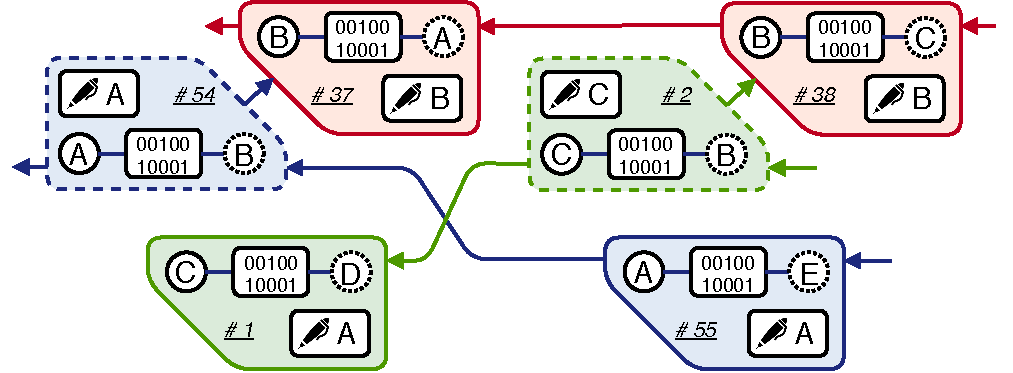
\includegraphics[width=.9\linewidth]{trustchain/assets/fullchain}
	\caption{A part of the \ModelName{} DAG with five users and six records: four proposals and two confirmations (indicated by dashed borders). The proposal created by user $ A $ is unconfirmed.}
	\label{fig:fullchain}
\end{figure}

\section{Detecting Fraud}
\label{sec:detecting_fraud}
We require that \ModelName{} detects malicious tampering of the records in a personal ledger.
\ModelName{} is built around fraud \emph{detection} instead of \emph{prevention}.
We argue this is a reasonable assumption for two reasons.
First, decentralized applications do not require the prevention of fraud~\cite{krishnan2002virtual}.
Fraud prevention is desired when the system manages monetary value, which is not the case when considering work accounting.
Second, preventing fraud is often a resource-intensive process that requires users to reach a consensus on all created records, e.g., using classical BFT algorithms or Proof-of-Work~\cite{vukolic2015quest}.
The requirement to reach consensus would severely limit the scalability and applicability of \ModelName{}.

%First, we highlight how an adversary would commit fraud in \ModelName{}.
Fraud in \ModelName{} proceeds when an adversary branches (or forks) its personal ledger and operates multiple personal ledgers in secret, possibly with a common prefix of records.
This fraud, for example, happens when an adversary attempts to hide a specific record by replacing it with another one.
This would result in pairs of records with the same sequence number and the same creator, but with a different hash.
The adversary can then return conflicting records to distinct peers.
A key objective of \ModelName{} is to quickly detect such conflicting records.
%This fraud model aligns with related work on free-riding behaviour in peer-to-peer networks~\cite{haeberlen2007peerreview}.

%According to our threat model, manipulation in \ModelName{} involves an adversary maintaining two different personal ledgers, possibly with a common prefix.
%In related literature, this is often referred to as double-spending or chain forking.

%To incentivize users to participate in the exploration of the \ModelName{} DAG, we propose that collected fraud proofs can be given to resource providers to gain preferential treatment.\todo{elaborate}
%For example, a user $ A $ can modify, reorder or remove micro-records in their personal ledger, and recompute the hash pointers to restore validity.
%However, this basic manipulation can be proven by interaction partners of $ A $ by having them broadcasting the original and manipulated micro-records created by $ A $ with the same sequence number.

%To prove this fraud to others, a user can broadcast the original and manipulated micro-records.

\begin{figure*}[t!]
	\centering
	\begin{subfigure}[t]{.5\textwidth}
		\centering
		\captionsetup{width=.9\linewidth}
		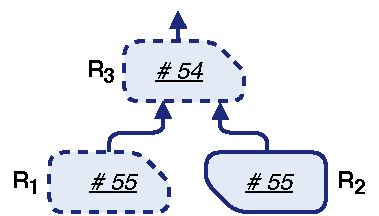
\includegraphics[width=.75\linewidth]{trustchain/assets/fraud_scenario_1}
		\caption{\emph{Scenario I}: $ R_1 $ and $ R_2 $ have the same sequence number but a different hash. this provides an irrefutable proof of fraud.}
		\label{fig:fraud_scenario_1}
	\end{subfigure}%
	\begin{subfigure}[t]{.5\textwidth}
		\centering
		\captionsetup{width=.89\linewidth}
		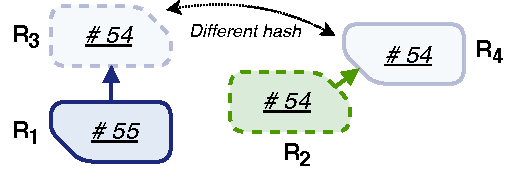
\includegraphics[width=.75\linewidth]{trustchain/assets/fraud_scenario_2}
		\caption{\emph{Scenario II}: $ R_1 $ and $ R_2 $ point to a record with the same sequence number and creator, but a different hash. This reveals an inconsistency.}
		\label{fig:fraud_scenario_2}\vspace{0.9cm}
	\end{subfigure}
	\begin{subfigure}[t]{.5\textwidth}
		\centering
		\captionsetup{width=.89\linewidth}
		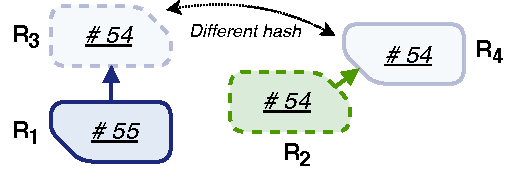
\includegraphics[width=\linewidth]{trustchain/assets/fraud_scenario_3}
		\caption{\emph{Scenario III}: $ R_1 $ and $ R_2 $ point to a record with the same sequence number and creator, but a different hash. This reveals an inconsistency.}
		\label{fig:fraud_scenario_3}\vspace{0.9cm}
	\end{subfigure}
	\begin{subfigure}[t]{.6\textwidth}
		\centering
		\captionsetup{width=.93\linewidth}
		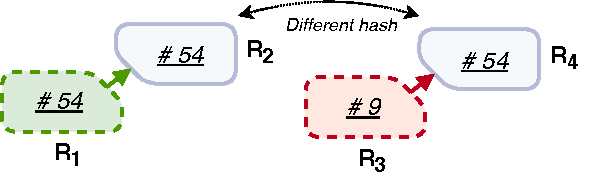
\includegraphics[width=.98\linewidth]{trustchain/assets/fraud_scenario_4}
		\caption{\emph{Scenario IV}: $ R_1 $ and $ R_3 $ confirm a record with the same sequence number and creator, but a different hash. This reveals an inconsistency.}
		\label{fig:fraud_scenario_4}
	\end{subfigure}
	\caption{Four scenarios which allows a peer to either expose fraud (forking of a personal ledger), or to detect an inconsistency. The colour of each record indicates the identity of its creator (blue for $ a $, green for $ b $ and red for $ c $). Solid and dashed records indicate proposals, respectively confirmations. Opaque records are not in possession by the peer.}
	\label{fig:fraud_scenarios}
\end{figure*}

\subsection{Detecting Forks}
\label{sec:detecting_forks}
Fraud in \ModelName{} is detected by sharing records with random peers, and by verifying the consistency of included hash pointers in these incoming records against known ones.
%In \ModelName{}, users continuously request micro-records in the personal ledger of other users, and the micro-records that confirm the requested micro-records.
This simple approach enables quick fraud detection through the collective effort of peers.
%When a user refuses to send requested micro-records to a requester within reasonable time, the requester blacklists that user and refuses to share resources with that user.
In Figure~\ref{fig:fraud_scenarios}, we visualize four identified scenarios in which we can either expose an adversarial peer (scenario I and II), or detect an inconsistency without assigning blame (scenario III and IV).
Each scenario shows records that a peer has in its local database, or does not have.
Records not in the possession by a peer are faded.
Records with the same colour are created by the same peer.
We discuss each scenario and elaborate how they lead to either fraud exposure or inconsistency detection.

\begin{itemize}
	\item \textbf{Scenario I}. 
	The first scenario, visualizes in Figure~\ref{fig:fraud_scenario_1}, captures the situation where a peer can directly expose a fork in ones personal ledger.
	This personal ledger in Figure~\ref{fig:fraud_scenario_2} has been forked since record $ R_1 $ and $ R_2 $ have the same sequence number but a different hash.
	As soon as another peer, say $ b $, receives $ R_1 $ while already having $ R_2 $, or receives $ R_2 $ while already having $ R_1 $, the pair $ (R_1, R_2) $ is sufficient evidence to expose the fraud by $ a $ and to prove that $ a $ has forked its personal ledger.
	Note that $ b $ does not need to have $ R_3 $ to detect or prove this fraud.
	We call the pair $ (R_1, R_2) $ a \emph{fraud proof}.
	Fraud proofs are by default shared within a \texttt{FraudProof} message with other peers in the \ModelName{} network.
	\item \textbf{Scenario II}. The second scenario describes the situation where one can prove fraud through the hashes in the prior pointer set $ S $.
	Figure~\ref{fig:fraud_scenario_2} shows four records created by the same peer.
	Records $ R_3 $ and $ R_4 $ contain the hash of the record with sequence number 54 in $ S $, however, they point to records with a different hash.
	The pair $ (R_3, R_4) $ can now be used to construct a fraud proof.
	\item \textbf{Scenario III}.
	Figure~\ref{fig:fraud_scenario_3} shows the scenario where a peer receives proposal $ R_1 $ and already has confirmation $ R_2 $, or receives confirmation $ R_2 $ while already having proposal $ R_1 $.
	The peer does not have $ R_3 $ and $ R_4 $.
	The hash pointer to the prior record in $ R_1 $ differs from the hash pointer in the confirmation $ R_2 $.
	This indicates an inconsistency that is either introduced by user $ a $ forking its personal ledger at height 54, or by $ b $ having included an invalid hash pointer in $ R_2 $.
	A peer that encounters this situation during the validation optimistically sends the pair $ R_1 $ and $ R_2 $ within a \texttt{Inconsistency} message to other peers.
	\item \textbf{Scenario IV.}
	Figure~\ref{fig:fraud_scenario_3} highlights another scenario where a user encounters two confirmations ,$ R_1 $ and $ R_3 $, created by different users, that point to a record with the same public key and sequence number, but a differing hash.
	This either indicates a fork of the personal ledger of $ a $, or it can be the result of an invalid pointer in one of the confirmations.
\end{itemize}

%The other two scenarios, displayed in Figure~\ref{fig:fraud_scenario_2} and Figure~\ref{fig:fraud_scenario_3}, enables the detection of an inconsistency but one cannot assign blame without more context.

%A more advanced manipulation is \emph{forking}, where a user creates two micro-records with the %same sequence number but with different counterparties.
%The goal of this fraud is to hide a specific micro-record from ones personal ledger, e.g., records that indicate some resource consumptions.
%This is similar to the double-spend attack in blockchain ledgers like Bitcoin~\cite{grunspan2018double}.
%Only when a user discovers both conflicting micro-records, this manipulation can be proven.
%In Section~\ref{sec:fraud_detection_experiment} we demonstrate that this fraud can be detected within seconds.
%To prove this fraud, the transaction counterparty reveals both the correct block and the invalid block created by $ A $.

\begin{algorithm}[!t]
	\label{alg:record_data_validation}
	\caption{The validation of the fields in record $ R $.}
	\begin{algorithmic}[1]
		\Procedure{validateRecordFields}{$ R $}  \Comment{Step 1}
		\State $ valid \leftarrow $ true
		\If{$ R.seqNum < 1 $}
		\State $ valid \leftarrow $ false
		\EndIf
		
		\If{\textsc{isConfirmation($ R $)} \textbf{and} $ R.linkInfo.seqNum < 1 $}
		\State $ valid \leftarrow $ false
		\EndIf
		
		\If{\textbf{not} \textsc{publicKeyIsValid}($ R.pubKey $)}
		\State $ valid \leftarrow $ false
		\EndIf
		
		\If{\textbf{not} \textsc{signatureIsValid}($ R.pubKey $, $ R.sig $)}
		\State $ valid \leftarrow $ false
		\EndIf
		
		\If{\textbf{not} \textsc{publicKeyIsValid}($ R.pubKeyOther $)}
		\State $ valid \leftarrow $ false
		\EndIf
		
		\If{$ R.seqNum = 1 $ \textbf{and} $ R.prevHash \not= \bot $}
		\State $ valid \leftarrow $ false
		\EndIf
		
		\State \Return valid
		\EndProcedure
		
	\end{algorithmic}
\end{algorithm}

\subsection{Record Validation Logic}
\label{sec:validation_logic}
Based on the four scenarios identified in Section~\ref{sec:detecting_forks}, we devise and describe the validation logic of an incoming record $ R $.
Each peer keeps track of known hashes in a dictionary named \texttt{knownHashes}.
The key of this dictionary is a tuple with the public key and sequence number of records, and the value of dictionary entries is the hash of the record.
%To simplify the validation logic, proposals and confirmations have the same fields.
%The confirmation pointer is implemented with three fields: \textsc{linkPublicKey}, \textsc{linkSeqNum} and \textsc{linkHash}.
%In a proposal, these fields are set to \textsc{null}.
%Each user maintains a dictionary \textsc{hashes} with known hashes.
The validation logic of incoming records consists of the following five steps.

\begin{algorithm}[t]
	\label{alg:record_validation_step3}
	\caption{Validating an incoming record against a linked record.}
	\begin{algorithmic}[1]
		\Procedure{validateLink}{R}  \Comment{Step 3}
		\State $ linked \leftarrow db $.\textsc{getLinked(R)}
		\If{$ linked = \bot $}
		\State \Return true
		\EndIf
		\State
		\State $ proposal \leftarrow linked $ \textbf{if} \textsc{isConfirmation(R)} \textbf{else} $ R $
		\State $ confirmation \leftarrow linked $ \textbf{if} \textsc{isConfirmation($ linked $)} \textbf{else} $ R $
		\State
		\If{$ confirmation.pubKeyOther \not= proposal.pubKey $}
		\State \Return false
		\EndIf
		\If{$ confirmation.linkInfo.seqNum \not= proposal.seqNum $}
		\State \Return false
		\EndIf
		\If{$ confirmation.linkInfo.hash \not= proposal.hash $}
		\State \Return false
		\EndIf
		\State $ linkLinked \leftarrow $ db.\textsc{getLinked(}$ linked $\textsc{)}
		\If{$ linkLinked \not= \bot $ \textbf{or} $ link\_linked \not= R $}
		\State \Return false
		\EndIf
		\State \Return true
		\EndProcedure
	\end{algorithmic}
\end{algorithm}

\textbf{Step 1.}
We first verify the validity of the data elements included in $ R $.
This is performed by the \textsc{validateRecordFields} procedure, which returns a boolean value indicating if the record is well-structured or not.
Its implementation can be found in Listing~\ref{alg:record_data_validation}.
This step validates the sequence number (line 3), the included public keys (line 7 and 11), and the digital signature (line 9).
If the incoming record is a confirmation, it verifies that the sequence number in the \texttt{linkInfo} attribute is within a valid range (line 5).
It also checks whether the hash of the prior record is sane when the record is the first in ones personal ledger (line 13).
Any error in the included data elements of $ R $ is computationally efficient to detect and is likely to be the result of a software bug.

\textbf{Step 2.}
Next, we query the database for a record with the same public key and sequence number as the incoming record $ R $.
If such a linked record $ R' $ is in the database, we check the equality of $ R $ and $ R' $ by doing a pairwise comparison of all included data elements.
If $ R \not= R' $, we have detected a fork in the personal ledger of the creator of $ R' $.
We then share the fraud proof $ (R, R') $ with other peers in the network.
We detect the inconsistency described by scenario I during this step.

\textbf{Step 3.}
Next, we compare incoming record $ R $ with its counterpart, if available in the database.
This step is performed by the the \textsc{validateLink} procedure, outlined in Listing~\ref{alg:record_validation_step3}.
We first get the linked record from the database (line 2) and only continue with this validation step if we have this record in the database.
If $ R $ is a proposal, the linked record must be a confirmation and vice versa.
We check whether the public keys included in the proposal and confirmation are consistent (line 9), and verify the consistency of the \texttt{linkInfo} attributes in the confirmation (line 11-14).
We detect the inconsistency described by scenario III during this step (line 15-17).

\textbf{Step 4.}
Next, we verify if the pointers in the incoming record are consistent with known ones.
This is performed by the \textsc{validateLedgerLinks} procedure which implementation is given in Listing~\ref{alg:record_validation_step4}.
This procedure first checks whether the \texttt{prevHash} attribute in $ R $ is consistent with the information in the \texttt{knownHashes} dictionary (line 3).
We then iterate over the included back-pointers and verify their consistency with the entries in the \texttt{knownHashes} dictionary (line 6-10).
We detect the inconsistency described by scenario II during this step.

\textbf{Step 5.}
Finally, we verify the validity of the included payload, which is an application-dependent validation procedure.
As we will further outline in Section~\ref{sec:system_architecture}, shared-resource applications using \ModelName{} should implement a \emph{validation} policy that denote whether the payload of an incoming micro-record is valid in the context of the application.

\begin{algorithm}[t]
	\label{alg:record_validation_step4}
	\caption{Validating the consistency of pointers in an incoming record with known ones.}
	\begin{algorithmic}[1]
		
		\Procedure{validateLedgerLinks}{R}  \Comment{Step 4}
		\State $ hash \leftarrow knownHashes[(R.pubKey, R.seqNum - 1)] $
		\If{$ hash \not= \bot $ \textbf{and} $ hash \not= R.prevHash $}
		\State \Return false
		\EndIf
		\State
		\For{$ seqNum, hash $ \textbf{in} $ R.backPointers $}
		\State $ known \leftarrow knownHashes[(R.pubKey, seqNum)] $
		\If{$ hash \not= \bot $ \textbf{and} $ hash \not= R.prevHash $}
		\State \Return false
		\EndIf
		\EndFor
		\State \Return true
		\EndProcedure
		
	\end{algorithmic}
\end{algorithm}

\subsection{Exchanging Records with Other Peers}
\label{sec:exchanging_records}
The detection of fraud requires adequate strategies to exchange records between other peers in the network.
\ModelName{} relies both on a \emph{push-based} and a \emph{pull-based} exchange of records.

\textbf{Pull-based Record Exchange.}
Each peer by default requests (pulls) records from other random peers at a fixed rate by sending out \texttt{Query} messages.
Applications can choose to send out \texttt{Query} messages to specific peers to build profile information about that peer, e.g., to detect free-riders.
A \texttt{Query} message contains a list of sequence numbers that the recipient should send back.
When receiving a \texttt{Query} message, the recipient includes linked proposal or confirmation records in the response.
When a peer does not answer with records within reasonable time, a requesting peer adds $ a $ to the blacklist managed by the connected application.

\textbf{Push-based Record Exchange.}
\ModelName{} also supports push-based record exchange, where the creator of a record disseminates it to $ f $ random other peers (as discussed in Section~\ref{sec:recording_interactions}).
This push-based exchange allows for quick detection of forking since the probability of no user receiving two conflicting records quickly goes to zero, even when the network size increases~\cite{osipkov2007combating}.
Furthermore, immediately disseminating a record in the network helps with record availability in case peers go offline.

\begin{figure*}[t]
	\centering
	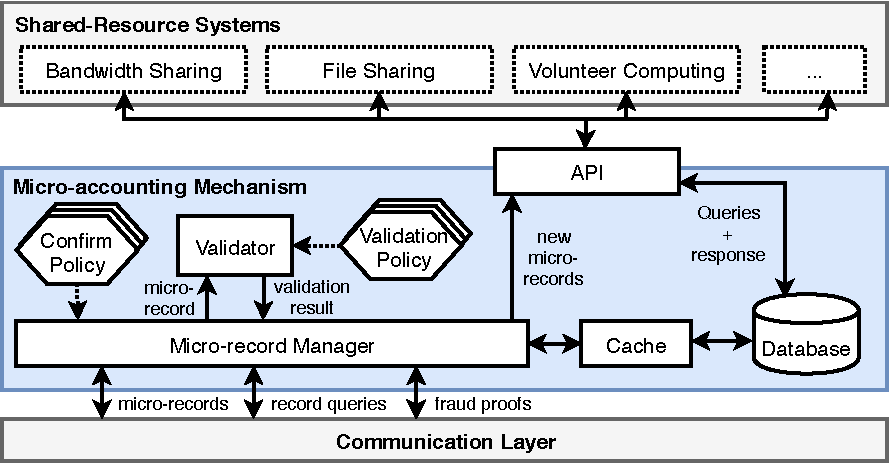
\includegraphics[width=\linewidth]{trustchain/assets/system_architecture}
	\caption{The system architecture of \ModelName{}.}
	\label{fig:system_architecture}
\end{figure*}

\section{System Architecture}
\label{sec:system_architecture}
%We present the components of our middleware, which is visualized in Figure~\ref{fig:system_architecture}.
%We consider peer-to-peer communities without centralized server.
%We also deem threats at the network layer, such as the Sybil Attack and the Eclipse Attack, outside scope of this work.

%\subsection{Underlying Model for Resource Management}
%Figure~\ref{fig:model} shows the underlying model of our middleware.
%This model is inspired by prior work on deterring free-riders in BitTorrent networks based on reputation, and consists of three components~\cite{seuken2010accounting,meulpolder2009bartercast}.
%An \emph{accounting mechanism} (see Section X) stores all resource contributions and consumptions by agents.
%These actions are embedded in tamper-proof and light-weight records, and shared with other individuals in the network.
%Each individual collects records from others, eventually building a local database.
%These records are then passed to a \emph{reputation algorithm} that determines the trustworthiness of individuals it knows about.
%Even though accounting mechanisms and reputation mechanisms share similarities, they are incomparable as discussed in the work of Seuken et al.~\cite{seuken2010accounting}.
%There exists a large number of decentralized reputation algorithm.
%The output of the reputation algorithm is a mapping from the identity of individuals to a trust score.
%These trust scores are used by the \emph{allocation policy} to provide access to some common good.
%The interactions following the allocation are accounted and public, and influence subsequent trust scores.
%For example, if a peer $ A $ downloads from another peer $ B $, the trust score of peer $ B $ most likely increases whereas the scores of peer $ A $ decreases.

We devise a system architecture around our \ModelName{} data structure (see Figure~\ref{fig:system_architecture}) and elaborate its components.
%We also demonstrate how resource-sharing applications can leverage the described system architecture and leverage \ModelName{} for resource accounting.
The network layer is the lowest layer in our architecture and provides the primitives for decentralized communication and messaging.
This layer can be realised using existing frameworks to build peer-to-peer overlay networks, e.g., libp2p.\footnote{See \url{https://libp2p.io}}
%Mitigation of network threats, e.g., the Sybil and Eclipse attacks, should be addressed by the communication layer.

\textbf{Record Manager.}
The record manager interacts with the network layer to disseminate records and to process incoming ones.
It queues incoming records for validation and persists incoming fraud proofs to the database.
It also manages the confirmation of incoming, valid proposal records that are targeted at that peer.
Applications using \ModelName{} should provide a \emph{confirmation policy} that predicates whether an incoming proposal should be confirmed.
%When micro-records arrive from the network, the record manager first checks if it has been received before.
%If not, it schedules the micro-record for validation.

\textbf{Validator.}
The validator assesses the validity of incoming records according to the algorithms described in Section~\ref{sec:validation_logic}.
%We distinguish between validation on \emph{record-level} and \emph{data-level}.
%Validation on record-level verifies the whether the micro-record itself is valid, e.g., whether it contains a valid digital signature and whether the micro-record is in alignment with other known micro-records in the personal ledger.
%These validation rules are application-agnostic.
%Validation on data-level verifies integrity of the micro-record with respect to an application context.
%Note that the validator might not have sufficient information to validate an incoming micro-record on data-level and therefore must collect more micro-records first.
Connection applications can provide a custom \emph{validation policy}.
If implemented, this validation policy is invoked during step 5, when the application-specific payload is validated.
The flexibility to provide custom validation and confirmation policies makes \ModelName{} universal and reusable across different application domains.

%\begin{algorithm}[b]
%	\SetAlgoLined
%	\small
%	\KwData{Micro-record \emph{R}, database \emph{db}}
%	\lIf{$ R $.$sequence\_number < 1 $}{\Return{} \textbf{false}}
%	\lIf{f}{\Return{} \textbf{false}}

%	\caption{The validation of a micro-record}
%\end{algorithm}

\textbf{Persistence.}
Records and fraud proofs are persisted in a database.
The \ModelName{} system architecture provides an interface for the queries made to the database and supports different database architectures, e.g., structured or unstructured storage models.
All query databases by \ModelName{} are routed through a \emph{cache}, which is an intermediary component that pre-loads all records in the personal ledger of the operating peer.
This allows \ModelName{} to quickly respond to incoming record queries.
%Micro-records of ones own personal ledger are cached in an intermediary \emph{record cache} in order to quickly respond to incoming queries.
%The record cache stores intermediate records for quick lookup when receiving a query for micro-records in ones personal chain.
%When initiating \ModelName{}, it pre-loads the micro-records of the operating user in the cache.
This cache interacts with the database for the retrieval and storage of records and fraud proofs.

To limit the growth of the database and to keep the storage overhead manageable, an application can choose to periodically prune the database when it reaches a storage threshold.
In our implementation, we start pruning when at least 1 million records have been stored.
Applications may increase or decrease this number, depending on the storage capacities of participating peers.
The default pruning strategy of \ModelName{} continuously removes the record with the lowest database insertion timestamps, until the database size has reached its storage threshold again.
The pruning of older records might cause some forks to go undetected, since records are removed before a fraud proof can be constructed.
As we will show in Section~\ref{sec:fraud_detection_experiment}, forks in \ModelName{} are quickly detected and there should be ample time to detect inconsistencies before relevant records are removed.

\textbf{Fraud Management.}
When the validator exposes fraud, or when it receives an incoming fraud proof, the connected applications are notified of the event and can punishment the misbehaving peer accordingly.
For example, a fraud policy in a bandwidth sharing application could decide to not serve the fraudster for some time.
The decentralized application should store the digital identities of fraudsters in a local blacklist.

%Despite enforcing a temporal order in a personal ledger, there is no notion of physical event time in \ModelName{}.
%Even if we would extend micro-records with a timestamp field, there is no guarantee that the included timestamp is accurate.
%This inaccuracy prevents resource-sharing applications using \ModelName{} to utilize time-based policy, e.g., banning adversarial users for 24-hours after the moment the fraud has been committed. % have committed fraud.
%In a distributed system with Byzantine actors, it is not practically possible to accurately synchronize time.
%Even though we consider accurate timestamping of events out of scope, we briefly outline two solutions.
%One approach is to use Proof-of-Work mechanisms to implement a distributed timestamp service.
%However, this approach is resource intensive and there would still be inaccuracies in the produced timestamps.
%Alternatively, one can use a third-party timestamping service and include their signature in the payload of a micro-record.
%However, this would violate our requirement for full decentralization, as discussed in Section~\ref{sec:problem_description}.

\textbf{Interacting with \ModelName{} by Applications.}
Decentralized applications interact with \ModelName{} through an API.
This API allows connected applications to query the content of the database.
Furthermore, connected applications can subscribe to incoming records.
The record manager forwards new records to the API, which passes these records to subscribed application.

\begin{table}[]
	\begin{center}
		\begin{tabular}{l l}
			\hline
			\textbf{Parameter} & \textbf{Default Value}  \\ \hline
			Peers ($ n $) & 1'000 \\
			Workload & 1 proposal per second per peer \\
			Record exchange strategy & \texttt{PULL+RAND+PUSH} \\
			Record fanout ($ f $) & 5 \\
			Crawl batch size & 2 \\
			Crawl interval & 0.5 seconds \\
			Packet Loss Rate & 0\% \\
			Individual forking probability & 10\% \\
			Back-pointers ($ b $) & 10 \\ \hline
		\end{tabular}
		\caption{The default parameters used during our evaluation.}
		\label{tab:experiment_parameters}
	\end{center}
\end{table}


\section{Implementation and Evaluation}
\label{sec:implementation_evaluation}
We implement \ModelName{} in the Python 3 programming language.
We leverage an existing library as network layer and use the UDP protocol for network communication.\footnote{See \url{https://github.com/tribler/py-ipv8}}
Our implementation uses the \texttt{asyncio} framework for asynchronous event handling.
Furthermore, it features both an (optimized) in-memory storage and a persistent \texttt{sqlite} database.
The full implementation of \ModelName{}, including unit tests and documentation, is published on GitHub.\footnote{See \url{https://github.com/tribler/py-ipv8/tree/master/ipv8/attestation/trustchain}}

\subsection{Experiment Setup}
We evaluate the impact of different parameters in \ModelName{} on the efficiency of fraud detection.
We do so by measuring the time between committing the fraud and its initial detection.
We substitute our networking layer with the SimPy discrete event simulator~\cite{matloff2008introduction}.
Each peer in the \ModelName{} network knows the network address of 100 random other peers, resulting in an unstructured overlay topology.
Table~\ref{tab:experiment_parameters} lists the default parameters during our experiments, unless stated otherwise.
To encourage reproducibility, we have open-sourced the \ModelName{} simulator and all experiment scripts\footnote{See \url{https://github.com/devos50/trustchain-simulator}}.

\textbf{Workload and Attack Model.}
During our experiments, peers create records with other random peers.
With our default workload, each peer initiates one proposal per second with another random peer in the network.
Note that the rate at which new records are created grows with the network size, which should capture the dynamics within real-world applications.
Each peer forks its personal ledger with a probability of 10\% by removing the last record in its personal ledger and re-using its sequence number to create a new record.
Each peer commits this fraud once.
A peer committing fraud will not broadcast the duplicate record when push-based record exchange is enabled.
In each experiment run, all peers start with an empty personal ledger, and interaction partners always confirm incoming proposals.
A peer that has exposed the fraud by another peer will refuse to confirm the proposals by that peer.
Each experiment run terminates either when all fraud attempts have been discovered or after ten minutes have elapsed.

\textbf{Record Exchange Strategies.}
We consider the following four strategies for exchanging records.
With the \texttt{PULL} strategy, each peer requests two contiguous records at a random height in the personal ledger of another random user every half a second (the \emph{crawl batch size} and \emph{crawl interval} parameters in Table~\ref{tab:experiment_parameters}).
Under the \texttt{PULL+RAND}, a peer also returns five random records in their database upon a query.
Including random records in a crawl response enables the detection of fraud of offline peers.
The \texttt{PULL+PUSH} strategy also pushes new records to $ f $ random users upon creation.
Finally, we consider the \texttt{PULL+RAND+PUSH} record exchange strategy, which is a combination of the above techniques.

\begin{figure*}[t]
	\centering
	\begin{subfigure}{.8\columnwidth}
		\centering
		
\includegraphics[width=\linewidth]{trustchain/assets/fraud_experiments_legend}
	\end{subfigure}
	\begin{subfigure}{.5\columnwidth}
		\centering
		\captionsetup{width=.9\linewidth}
		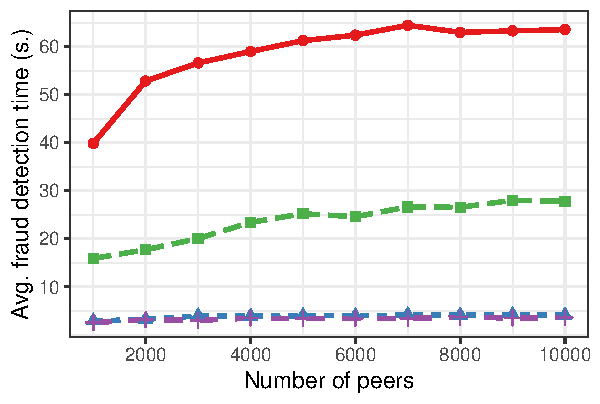
\includegraphics[width=\linewidth]{trustchain/assets/fraud_times_scalability}
		\caption{Average fraud detection times as the number of peers increases.}
		\label{fig:experiment_scalability_detection_times}
	\end{subfigure}%
	\begin{subfigure}{.5\columnwidth}
		\centering
		\captionsetup{width=.9\linewidth}
		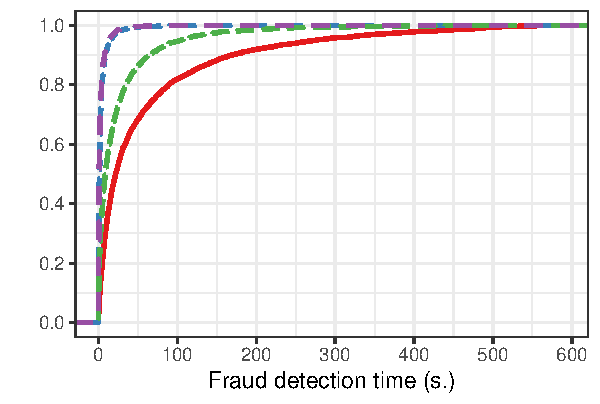
\includegraphics[width=\columnwidth]{trustchain/assets/fraud_times_scalability_5000_ecdf}
		\caption{The Empirical Cumulative Distribution Function (ECDF) for 5'000 peers.}
		\label{fig:experiment_scalability_ecdf_detection_times}
	\end{subfigure}
	\begin{subfigure}{.5\columnwidth}
		\centering
		\captionsetup{width=.9\linewidth}
		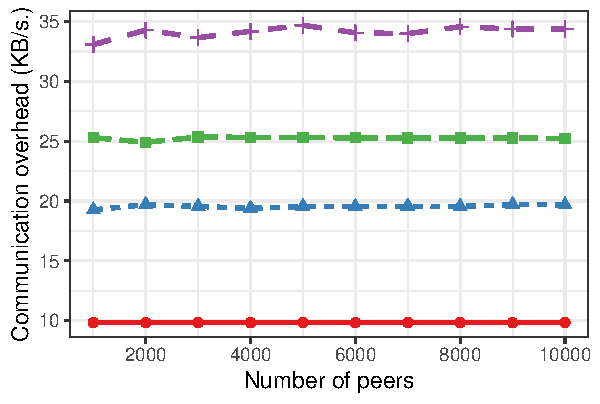
\includegraphics[width=\linewidth]{trustchain/assets/scalability_bandwidth_usage}
		\caption{Average network usage per peer as the number of peers increases.}
		\label{fig:experiment_scalability_bandwidth}
	\end{subfigure}%
	\begin{subfigure}{.5\columnwidth}
		\centering
		\captionsetup{width=.9\linewidth}
		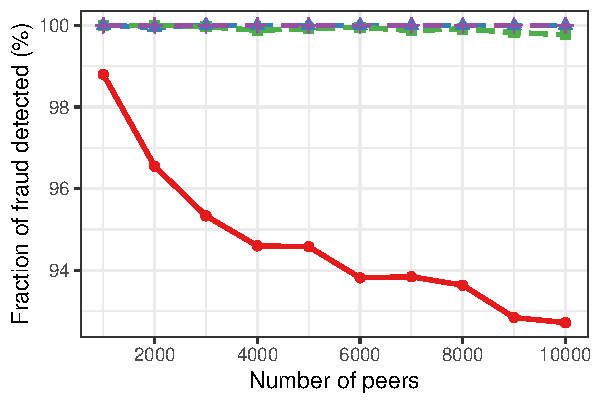
\includegraphics[width=\columnwidth]{trustchain/assets/scalability_num_detected}
		\caption{Fraction of fraud exposed after our experiment ends.}
		\label{fig:experiment_scalability_num_detected}
	\end{subfigure}
	\caption{The results of our scalability experiments, with up to 10'000 peers. We evaluate four record exchange strategies.}
	\label{fig:scalability_experiments}
\end{figure*}

\subsection{Scalability}
\label{sec:fraud_detection_experiment}
Our first experiment explores the scalability of \ModelName{} when increasing the number of peers in the network.
The results can be found in Figure~\ref{fig:scalability_experiments}.
Figure~\ref{fig:experiment_scalability_detection_times} shows the effect of increasing the number of peers on the average time until fraud detection, for different record exchange strategies.
For $ n = 10'000 $, the \texttt{PULL} strategy shows an average fraud detection time of 63.5 seconds, whereas this detection time decreases under the \texttt{PULL+RAND+PUSH} strategy to 3.6 seconds.
We notice that the \texttt{PULL+PUSH} and \texttt{PULL+RAND+PUSH} strategies show detection times under five seconds on average.
This demonstrates that disseminating a record just after its creation is a successful strategy.
Including random records in crawl responses also decreases detection times.
For $ n = 10'000 $, the average fraud detection time decreases from 63.5 seconds for the \texttt{PULL} strategy to 27.8 seconds for the \texttt{PULL+PUSH} strategy.

In Figure~\ref{fig:experiment_scalability_ecdf_detection_times} we show the The Empirical Cumulative Distribution Function (ECDF) of fraud detection times for $ n = 5'000 $.
We observe that it can take several minutes for some fraud attempts to be discovered, in particular when the \texttt{PULL} and \texttt{PULL+RAND} strategies are active.
Still, for the \texttt{PULL} strategy, we can detect 90\% of fraud attempts within 160 seconds and 50\% of the fraud attempts within 30 seconds.
We also observe that the vast majority of fraud is detected within a few seconds when pushing random records after creation.
82.9\% of all fraud attempts is detected within five seconds for the \texttt{PULL+RAND+PUSH} strategy.

Figure~\ref{fig:experiment_scalability_bandwidth} shows the average network usage per peer as the number of peers increases, for different record exchange strategies.
The \texttt{PULL} strategy requires less than 10KB per second of network usage.
Compared to the \texttt{PULL} strategy, the \texttt{PULL+RAND+PUSH} strategy uses over thrice as much bandwidth, around 35KB per second.
Note how the network usage remains roughly the same for all considered record exchange strategies as we add more peers to the experiment.
Figure~\ref{fig:experiment_scalability_bandwidth} shows that it is feasible to deploy \ModelName{} in consumer-grade network environments.
However, network usage can still be decreased by lowering the crawl interval and/or crawl batch size, at the cost of increased fraud detection times.

Not all fraud has been detected after our experiment has ended.
Figure~\ref{fig:experiment_scalability_num_detected} shows the percentage of fraud attempts that has been detected after the experiment has ended, for increasing number of peers and for different record exchange strategies.
It becomes less likely that fraud is detected during our experiment when increasing the network size under the \texttt{PULL} strategy.
For $ n = 10'000 $, 7.28\% of fraud attempts remain undetected.
These instances would likely be discovered when running the experiment longer.

%During the experiment, each peer explores others' personal ledgers by continuously querying their latest micro-record, and attempts to detect fraud.
%At the start of each experiment, we selected one peer to perform exactly one double spend attack.
%This peer re-uses the sequence number of the latest micro-record (forking) with 20\% probability.
%We measure the interval between initiation of the fraud and its first detection (upon which the proof can be spread in the network).
%We vary the rate at which users request micro-records from each other.
%We consider request frequencies of 5, 10 and 25 (where 5 means that each user will request a micro-record from five other users every second).
%For each combination of network size and ledger exploration rate, we run the experiment 20 times.

%Figure~\ref{fig:fraud_experiments_fixed_tx} shows the fraud detection times and bandwidth usage while recording 100 interactions per second, for different exchange strategies and network sizes ($ n $).
%Figure~\ref{fig:fraud_experiment_fixed_tx_time} reveals that fraud can be detected within ten seconds under all strategies, even when $ n = 1'000 $.
%The detection times decrease when enabling a push-based exchange strategy (\texttt{PULL+PUSH}), and when sharing random micro-records during a crawl (\texttt{PULL+RAND}).
%Furthermore, the detection times increase roughly linearly when increasing the network size for the \texttt{PULL+PUSH} and \texttt{PULL+RAND+PUSH} strategies.
%In Figure~\ref{fig:fraud_experiment_detect_times_fixed_1000}, we show an ECDF of the detection times for different strategy and with $ n = 1'000 $.
%Note how 50\% of all fraud attempts is detected within ten seconds.
%We notice a significant effect of the push-based exchange strategy on the detection times.
%We explain this effect as follows: pushing created micro-records to random users lead to near-immediate detection of fraud when a user receives two conflicting micro-records.
%Figure~\ref{fig:fraud_experiment_fixed_tx_bw} shows the average bandwidth consumption of each user during our five-minute runs.
%The average bandwidth usage decreases when the network grows which is likely the result of fixing the rate at which new micro-records are created.
%With $ n = 1'000 $, the \texttt{PULL+RAND+PUSH} strategy requires 25KB/s. on average and the \texttt{PULL} strategy only requires 14.5 KB/s.

%Figure~\ref{fig:fraud_experiments_dynamic_tx} shows the detection times and bandwidth usage while scaling the number of recorded interactions with the network size.
%This results in a higher fraud detection times, as hinted by Figure~\ref{fig:fraud_experiment_dynamic_tx_time}.
%Still, fraud attempts are detected within reasonable time: even the \texttt{PULL} strategy enables fraud detection within 22 seconds on average.
%Figure~\ref{fig:fraud_experiment_detect_times_dynamic_1000} shows that the effect of individual strategies on fraud detection times is more pronounced under a dynamic micro-record creation rate.
%Additionally, Figure~\ref{fig:fraud_experiment_dynamic_tx_bw} shows that the average bandwidth usage remains roughly constant when increasing the network size, but slightly drops for $ n > 800 $.
%These experiments show that fraud can be detected efficiently with reasonable bandwidth usage.

%The results are given in Figure \ref{fig:fraud_experiment}.
%The horizontal axis denotes the network size and the vertical axis shows the time interval between performing the forking and its detection.
%The errors bars show one standard deviation of uncertainty.
%Figure \ref{fig:fraud_experiment} shows that faster querying of micro-records increases the speed of fraud detection, at the expense of increased resources usage (bandwidth and CPU utilization).
%We observe that the variation of fraud detection speed is higher when exploring personal ledgers at a lower rate.
%Interesting is that effectiveness of fraud detection shows comparable results when the network size increases.
%Our reasoning for this is as follows: although the specific double spend is more "hidden" in the network, there is also more ongoing effort to detect it.
%This experiment shows that forking of a personal ledger can be detected within mere seconds and 1'000 active peers.

\begin{figure*}[!t]
	\centering
	\begin{subfigure}{.8\columnwidth}
		\centering
		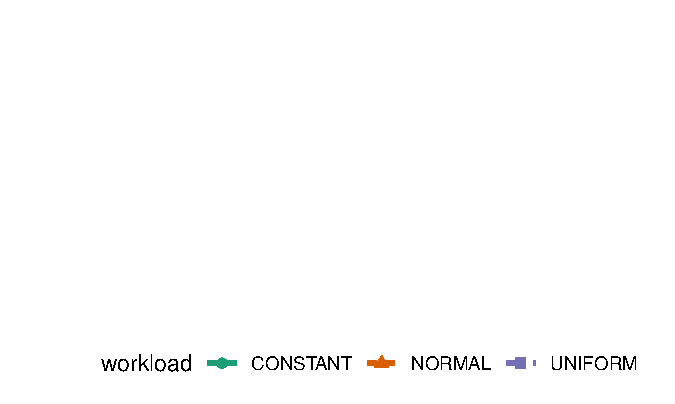
\includegraphics[width=.8\linewidth]{trustchain/assets/workloads_experiments_legend}
	\end{subfigure}
	\begin{subfigure}{.5\columnwidth}
		\centering
		\captionsetup{width=.9\linewidth}
		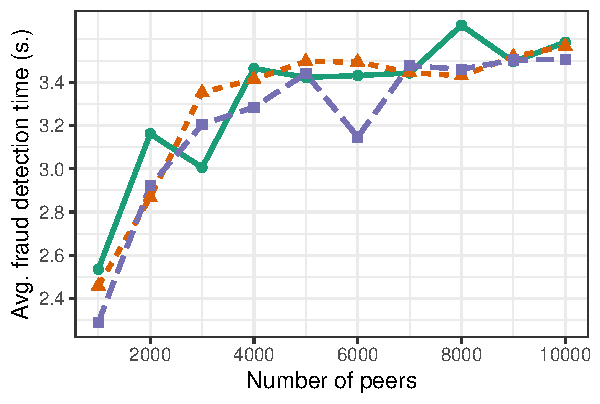
\includegraphics[width=\linewidth]{trustchain/assets/fraud_times_workloads}
		\caption{Average detection times as the number of peers increases.}
		\label{fig:workloads_experiment_fraud_detection_times}
	\end{subfigure}%
	\begin{subfigure}{.5\columnwidth}
		\centering
		\captionsetup{width=.9\linewidth}
		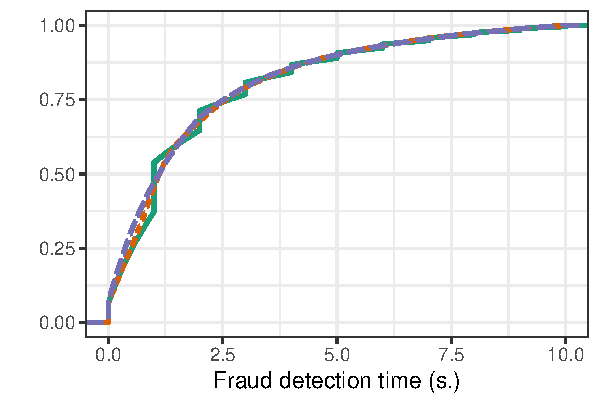
\includegraphics[width=\columnwidth]{trustchain/assets/fraud_times_workloads_5000_ecdf}
		\caption{The Empirical Cumulative Distribution Function (ECDF) of fraud detection times under ten seconds, for 5'000 peers.}
		\label{fig:workloads_experiment_ecdf_fraud_detection_times}
	\end{subfigure}
	\caption{Fraud detection times for different workload characteristics, up to $ n = 10'000 $.}
	\label{fig:workloads_experiments}
\end{figure*}

\subsection{Different Workloads}
Next, we evaluate the effect of different workloads on fraud detection times.
We consider three types workloads with differing rates at which new proposals are created.
In the \texttt{CONSTANT} workloads, peers create a new proposal record every second with another random peer.
Under the \texttt{UNIFORM} workload, the interval between creating new proposals is drawn from a uniform distribution $ \mathcal{U}(0, 2) $.
Under the \texttt{NORMAL} workload, this interval is drawn from a normal distribution $ \mathcal{N} $ with $ \mu = 1 $ and $ \sigma = 0.3 $.

The results are visualized in Figure~\ref{fig:workloads_experiments}.
Figure~\ref{fig:workloads_experiment_fraud_detection_times} shows how different workloads affect the average fraud detection times when the number of peers increases.
For all workloads, fraud attempts are detected within four seconds on average.
Fraud detection times are increasing for $ n \leq 5'000 $, but remains around 3.5 seconds for $ n > 5'000 $.
Figure~\ref{fig:workloads_experiment_ecdf_fraud_detection_times} shows the Empirical Cumulative Distribution Function (ECDF) of fraud detection times under ten seconds, for 5'000 peers.
For presentation clarity, we only consider fraud detection times under ten seconds.
Note how these workloads roughly lead to a similar distribution of fraud detection times.

\begin{figure}[t]
	\centering
	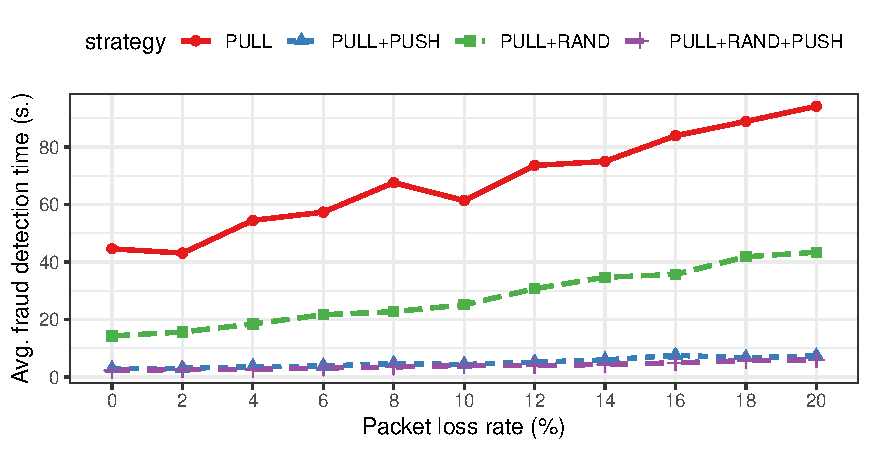
\includegraphics[width=.9\linewidth]{trustchain/assets/fraud_times_send_failure}
	\caption{The effect of packet loss on the average fraud detection times, for different record exchange strategies.}
	\label{fig:fraud_times_link_failures}
\end{figure}

\subsection{Packet Loss}
We explore the robustness of \ModelName{} by quantifying the effect of packet loss on the efficiency of fraud detection in \ModelName{}.
To this end, we increase the packet loss rate, up to 20\%, and run our simulations under different record exchange strategies.
Even though a packet loss rate of 20\% is an unlikely situation for environment in which \ModelName{} should be deployed, we are interested to see how robust \ModelName{} is, even in such extreme circumstances.
We expect the fraud detection times to increase when network stability is lower, since loosing packets makes it less likely to detect inconsistencies.

Figure~\ref{fig:fraud_times_link_failures} shows the average fraud detection times when increasing the packet loss rate, for our four record exchange strategies.
We observe that fraud detection times increase under the \texttt{PULL} and \texttt{PULL+RAND} strategies, whereas this effect is less for the \texttt{PULL+PUSH} and \texttt{PULL+RAND+PUSH} strategies.
Average fraud detection times under the \texttt{PULL} strategy increase from 44.6 seconds with no packet loss to 94.1 seconds when 20\% of all packets.
We notice that 23.8\% of all fraud attempts with a packet loss of 20\% and the \texttt{PULL} strategy remains uncovered after the experiment has ended.
This number is 0.2\% when no packets are lost.
For the \texttt{PULL+RAND+PUSH} strategy, this same increase is from 2.3 seconds to 6.0 seconds.
Under the \texttt{PULL+RAND+PUSH} strategy, we see that all fraud attempts are discovered in our experiment, for all evaluated packet loss rates.

\begin{figure}[t]
	\centering
	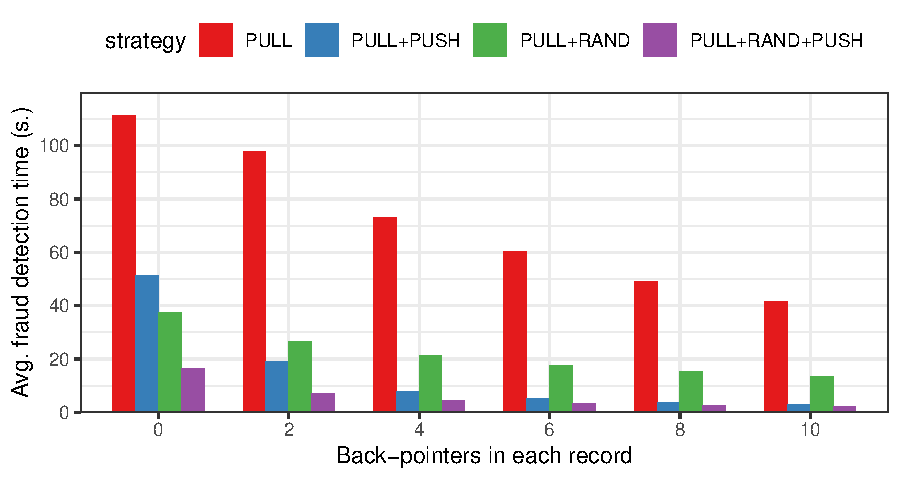
\includegraphics[width=.9\linewidth]{trustchain/assets/fraud_times_back_pointers}
	\caption{The effect of adding more back-pointers to each record on the average fraud detection times, for different record exchange strategies.}
	\label{fig:fraud_times_back_pointers}
\end{figure}

\subsection{Back Pointers}
We vary the number of back-pointers ($ b $) in each record and analyse the effect on the average fraud detection times.
We suspect that adding more back-pointers increases the probability of detecting fraud since individual records now bear more hashes of records in ones personal ledger.
This comes, however, at a cost of additional network usage and computational overhead to analyse the back-pointers.
Each back-pointer adds 32 bytes to the serialized record size.

The results are displayed in Figure~\ref{fig:fraud_times_back_pointers}, showing the number of back-pointers in each record on the horizontal axis and the average time until fraud is detected on the vertical axis, for different record exchange strategies.
Adding additional back-pointers indeed indeed decreases fraud detection times.
Under the \texttt{PULL} record exchange strategy, it takes 111.19 seconds to detect fraud when no additional back-pointers are included, whereas this time decreases to 41.6 seconds when adding up to ten back-pointers to each record, a decrease of 58.4\%.
This decrease is much more for the \texttt{PULL+PUSH} strategy, namely a decrease of 97\%.
Note that the effect of adding more back-pointers diminishes when increasing for $ b > 4 $.
This is can likely be attributed to the fact that all peers start with an empty personal ledger in our simulations, and that different records are more likely to include the same hashes in their back-pointers.
However, we believe that the effect of additional back-pointers becomes more apparent when personal ledgers grow to considerable sizes, since different records are then more likely to include unique hashes.

\subsection{Discussion}
The experiments in this section demonstrate that \ModelName{} is scalable, bandwidth efficient, and robust against packet loss.
We have also demonstrated the effect of different workloads and a varying number of back-pointers included in each record.
Even though we have not experimented with all parameters in Table~\ref{tab:experiment_parameters}, we believe that this set of experiments provides an adequate starting point for system designers to adopt and configure \ModelName{}.
With our open-source simulator, system designers can quickly analyse the effect of different parameters, potentially on a workload that matches with their application.

We have demonstrated that there is a trade-off between the average fraud detection times and network usage.
The acceptable network usage differs per applications, for example, bandwidth is likely to be less of a concern when considering a video streaming application than in an Internet-of-Things environment.
By reducing the crawl rates, fanout value, and back pointers, one can reduce the bandwidth footprint of \ModelName{}, at the cost of increased fraud detection times.
Figure~\ref{fig:experiment_scalability_bandwidth} shows that the active record exchange strategy also impacts network usage.
In a network with churn, we recommend to activate the \texttt{PULL+RAND} or \texttt{PULL+RAND+PUSH} strategies, where peers share random records in their database with others.
We recommend the \texttt{PULL+RAND+PUSH} strategy when fraud detection times must be low, and the \texttt{PULL} strategy when bandwidth is a limiting factor.

\section{Addressing Free-riding at Scale}
\label{sec:deployment}
To showcase the applicability of \ModelName{}, we conduct a large-scale deployment trial with to address free-riding behaviour in \Tribler{}, our decentralized file-sharing application~\cite{pouwelse2008tribler}.
\Tribler{} is downloaded by over 1.8 million users and features an onion-routing overlay that tunnels BitTorrent traffic through relay and exit nodes to provide anonymity.
Similar to Tor, these relay and exit nodes are operated by volunteers.
This network suffers from an undersupply of exit nodes, leading to frequent network congestions and an overall degradation of download speeds for all users.
We leverage \ModelName{} to account the performed work as relay or exit node, and the consumed work as downloader.
We then demotivate free-riding behaviour by offering users with higher net contributions preferential treatment during periods of congestion.

\subsection{Accounting Bandwidth Transfers}
With \ModelName{}, peers can earn \emph{bandwidth tokens} by forwarding traffic as a relay or exit node.
When a peer downloads content, the user compensates the used relay and exit nodes by paying them bandwidth tokens.
Figure~\ref{fig:payouts} show the dynamics of bandwidth tokens after a peer has downloaded a 50MB file over a two-hop circuit.
The downloader accounts a transfer of 250MB to the first relay using \ModelName{} (MB is the unit of this bandwidth token).
The first relay then transfers 150MB to the next relay node, resulting in a net positive of 100MB for the first relay.
The rationale behind our payout scheme is that we reward relay and exit nodes for performing the cryptographic work (e.g., encryption and decryption) on the forwarded data.
Relays that do not forward the payout to the next hop will be blacklisted by the previous hop, therefore lowering their opportunity to earn bandwidth tokens.
Each record in a personal ledger attached to the Tribler application contains both the token amount transferred, and the current token balance of the peer.
%We payout anonymous transfers of at least 1MB.

\begin{figure}[t]
	\centering
	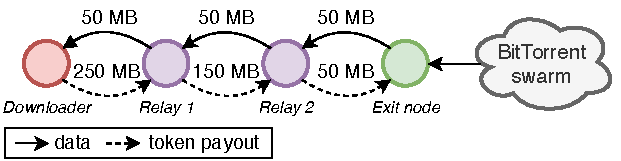
\includegraphics[width=.8\linewidth]{trustchain/assets/payouts}
	\caption{Accounting specifications of an anonymous 50MB BitTorrent download over a two-hop onion-routing circuit.}
	\label{fig:payouts}
\end{figure}

Since this use-case involves anonymous downloading, there is an important trade-off between accountability and anonymity.
We plan on addressing privacy concerns by having each node aggregate and delay payouts, a privacy-enhancing technique introduced in the work of Palmieri et al.~\cite{palmieri2015paying}.
Still, work accounting with \ModelName{} does not leak the identity of a downloader to other peers in the network, nor reveals any data being transferred over circuits.
To address the uncontrolled minting of bandwidth tokens by recording fake work, we are currently designing and implementing a Sybil-resistant reputation mechanism~\cite{otte2017trustchain}.

\begin{algorithm}[!t]
	\label{alg:slot_logic}
	\caption{The assignment logic of slots to circuits. $ N_{rand} $ and $ N_{comp} $ represent the maximum number of random and competitive slots, respectively.}
	\begin{algorithmic}[1]
		\State $ S_{rand} \leftarrow [\bot] * N_{rand} $ \Comment{array with circuit IDs}
		\State $ S_{comp} \leftarrow [(-\infty, \bot)] * N_{comp} $ \Comment{array with balances and circuit IDs}
		\State
		
		\Function{onCircuitRequest}{$ c $}
		\For{$ i = 0 $ to $ N_{rand} $}
		\If{$ S_{rand}[i] = \bot $}
		\Comment{Random slot is available}
		\State $ S_{rand}[i] \leftarrow c $
		\State \Return
		\EndIf
		\EndFor
		
		\State Query the balance of the initiator of $ c $
		
		\EndFunction
		\State
		
		\Function{onBalance}{$ c $, $ b $}
		\State $ B_{lowest} \leftarrow \infty $
		\State $ I_{lowest} \leftarrow \infty $
		\For{$ i = 0 $ to $ N_{comp} $}
		\If{$ S_{comp}[i] = (-\infty, \bot) $} \Comment{Competitive slot is available}
		\State $ S_{comp}[i] \leftarrow (c,b) $
		\State \Return
		\EndIf
		
		\If{$ S_{comp}[i][0] < B_{lowest} $}
		\State $ B_{lowest} \leftarrow S_{comp}[i][0] $
		\State $ I_{lowest} \leftarrow i $
		\EndIf
		\EndFor
		
		\If{$ b > B_{lowest} $}
		\State Destroy circuit stored in $ S_{comp}[I_{lowest}][1] $
		\State $ S_{rand} \leftarrow (c, b) $
		\EndIf
		
		\EndFunction
		
	\end{algorithmic}
\end{algorithm}

\subsection{Circuit Assignment}
We leverage the records created with \ModelName{} to grant preferential treatment to peers with higher token balances during periods of congestion.
Specifically, we modify the logic of relay and exit nodes such that each circuit consumes an available slot at their side.
The slot assignment logic is displayed in Listing as pseudocode~\ref{alg:slot_logic}.
We distinguish between \emph{random} and \emph{competitive} slots.
When a circuit initiation request arrives, the \texttt{onCircuitRequest} method is invoked and \Tribler{} first determines if there is a random slot available (line 5-9).
If so, we assign the new circuit to the random slot (line 7).
If no random slot is available, \Tribler{} queries the bandwidth token balance of the circuit initiator $ i $ by requesting the records in the personal ledger of $ i $.
When receiving these records, \Tribler{} determines the balance and checks eligibility for a competitive slot (line 12-23).
If there is an unoccupied competitive slot, \Tribler{} assigns the new circuit to it (line 16).
If all competitive slots are filled, the circuit of the initiator with the lowest amount of bandwidth tokens, say $ p $, is destroyed if the token balance of $ i $ is higher than the token balance of $ p $ (line 22).
This pre-emptive approach frees up the competitive slot for the circuit of $ i $.
As a result, users with a higher token balance have more chance to claim a competitive slot in periods of congestion, compared to free-riders, and experience higher and more stable download speeds.
We consider the analysis of different allocation policies, e.g., using a packet-granular scheduler, as further work.

%\begin{figure}[t]
%	\centering
%	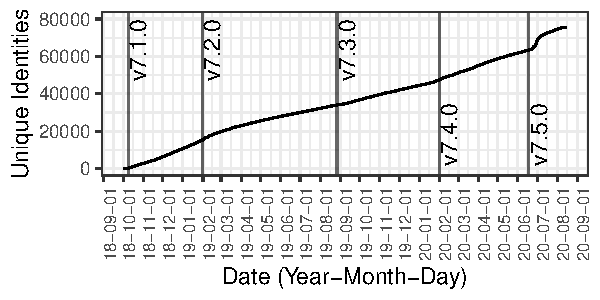
\includegraphics[width=\linewidth]{assets/identities_per_day}
%	\caption{ECDF showing the distribution of bandwidth token balances users and individual rejects events at exit nodes.}
%	\label{fig:identities_per_day}
%\end{figure}

\begin{figure}[!t]
	\centering
	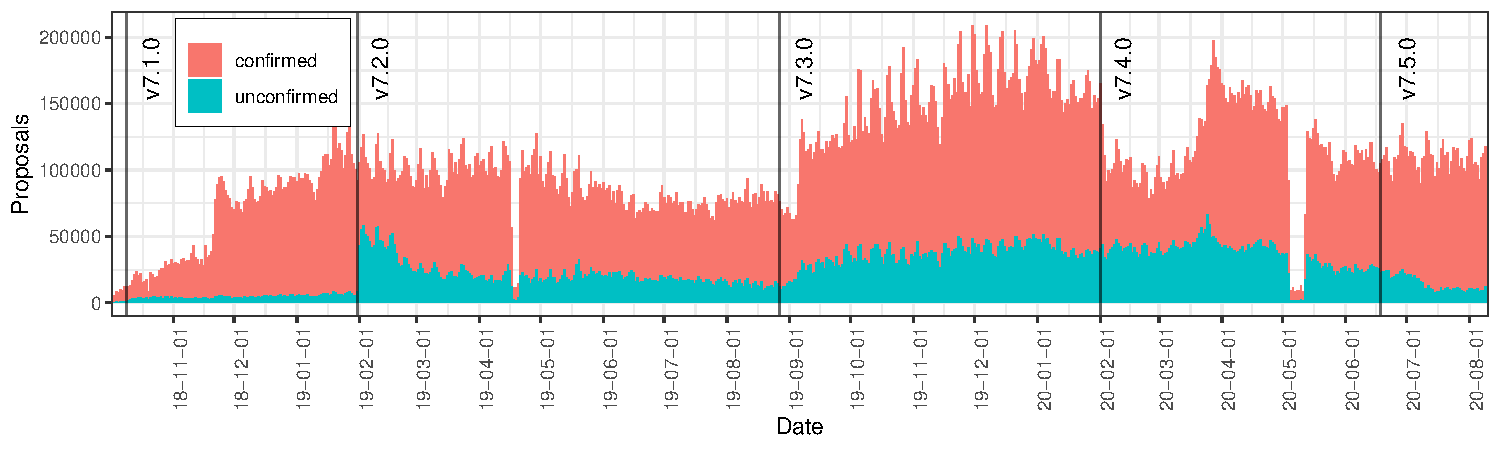
\includegraphics[width=\linewidth]{trustchain/assets/record_creation}
	\caption{Daily creation statistics of records, during a period of two years. We annotate the major releases of \Tribler{}.}
	\label{fig:record_creation}
\end{figure}

\subsection{Data Collection}
We integrate the accounting and slot mechanism in \Tribler{} and release a new version of our software.
We also deploy a crawler that continuously queries \ModelName{} records from random users in the \Tribler{} network.
Every two seconds, this crawler selects a random peer in the \ModelName{} network and requests missing records in their personal ledger.
A deployment period of two years has resulted in more than \TrialRecords{} records, created by over \TrialUsers{} peers.
Collected records are stored in a sqlite database that is enhanced with additional indices to speed up insertion and analysis.
The filesize of the database with all collected records is around 120GB, and we plan on releasing the full data set.
Our crawler also discovered 127'135 instances where a personal ledger was forked.
We find that 11.4\% of all collected proposals in the deployed \ModelName{} network is unconfirmed.
This is either because the proposal counterparty has not created a confirmation, or because our crawler has not picked up the confirmation record.

Monitoring the records created by \ModelName{} not only allows us to detect free-riders in \Tribler{} but also allows us to detect anomalies caused by software bugs or unexpected user behaviour.
It also enables us to monitor the growth of users within \Tribler{} by tracking the number of unique peers in the \ModelName{} network.
The inclusion of a timestamp in the payload of each record created by \ModelName{} also helps us to analyse network health and user behaviour.

Figure~\ref{fig:record_creation} shows the daily number of created proposal and confirmation records.
We also annotate the dates on which we released a major version of \Tribler{}.
Figure~\ref{fig:record_creation} shows that more users run \Tribler{} during the weekend and therefore create more proposals on a Saturday and Sunday.
We also observed two large-scale outage of exit nodes, in April 2019 and May 2020, likely due to infrastructure failure.
Despite this outage, users would still perform payouts when downloading directly from other \Tribler{} users, proving the robustness of \ModelName{}.
%Note how major release of \Tribler{} is not significantly resulting in an increased number of micro-records.

%In \Tribler{}, users earn bandwidth tokens by either operating an exit node, or by relaying traffic.
%By default, users download with one-hop anonymity, meaning that the circuit is directly connected to an available exit node.
%We noticed that only few users increase this setting since adding additional hops to a circuit negatively impacts the achievable download speed.
%There is a delicate trade-off between anonymity and download speed. 
%Therefore, there is an oversupply of relay nodes but the majority of users do not require a relay node for their downloads.
%Eventually, we aim to adjust the default number of hops for a download to two, increasing the opportunities for relay nodes to earn bandwidth tokens.
%We are currently improving the performance of our anonymous download mechanism.

\begin{figure}[t]
	\centering
	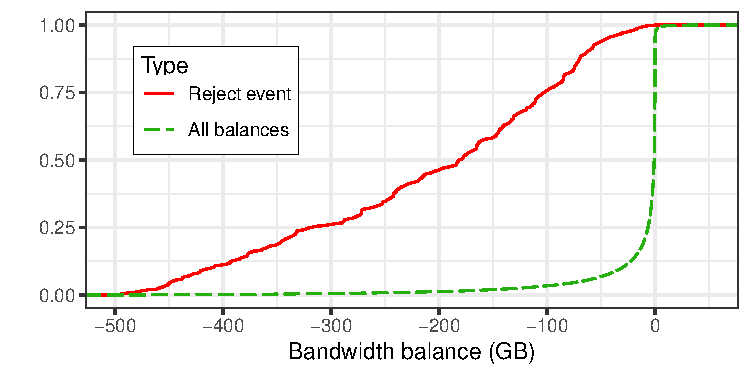
\includegraphics[width=.8\linewidth]{trustchain/assets/exit_node_rejects}
	\caption{Emperical Cumulative Distribution Function (ECDF) of the bandwidth token balances users and individual rejects events at exit nodes.}
	\label{fig:exit_node_rejects}
\end{figure}

\subsection{Free-rider Identification and Service Refusal}
To evaluate whether free-riding behaviour is addressed, we deploy 48 \Tribler{} exit nodes.
Each exit node is configured with a total of 10 random slots and 20 competitive slots, resulting in a total of 1'440 slots.
To obtain insights in the circuit assignment logic, we log the bandwidth token balance when a circuit initiator is unable to claim a competitive slot at one of our exit nodes.
In total, we logged over 1.4 million reject events during three weeks.

Figure~\ref{fig:exit_node_rejects} shows an ECDF with the bandwidth token balances of all users (dotted green line) and the balances associated with rejected circuit requests (solid red line).
We filter out all users and reject events with balances higher than 50GB or lower than -500GB.
The median token balance of all users is -713MB and that of reject events -181.4GB, demonstrating that our mechanism targets users with lower balances.
In other words, long-term free-riders are likely to be kicked out when the network is congested.
This deployment trial shows that \ModelName{} is effective at detecting and addressing free-riding behaviour in \Tribler{}.
On the long term, the integration of \ModelName{} increases network performance and induces fairness amongst downloading users.

%\begin{figure}[t]
%	\centering
%	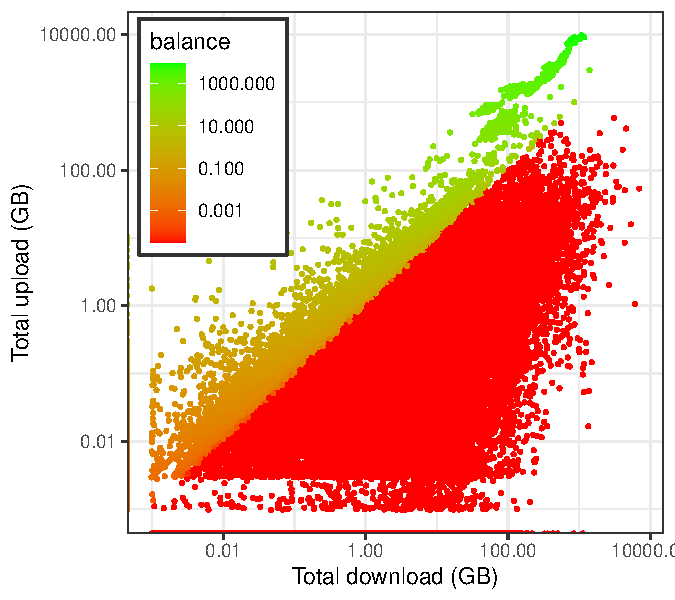
\includegraphics[width=\linewidth]{assets/balances_scatter}
%	\caption{The bandwidth balances of users in Tribler. Users with a balances less than 5GB are marked red.}
%	\label{fig:balances}
%\end{figure}

%\begin{figure}[t]
%	\centering
%	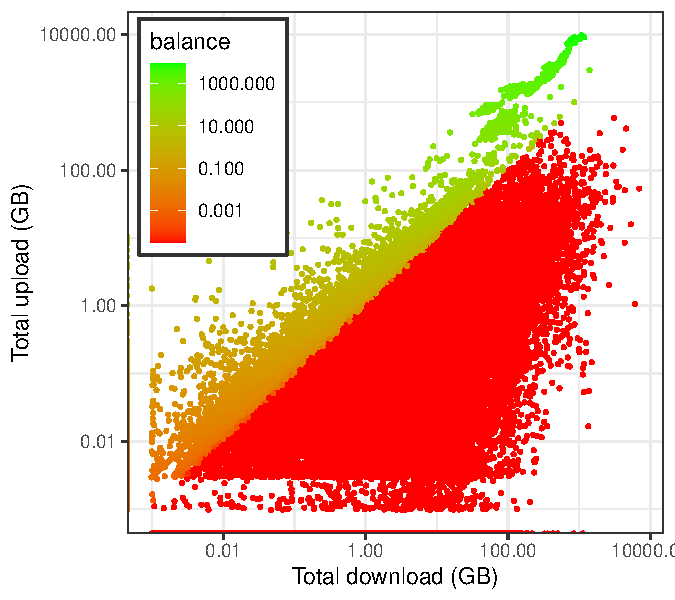
\includegraphics[width=\linewidth]{assets/balances_scatter}
%	\caption{Scatterplot of user balances where each point represents a user in \Tribler{}.}
%	\label{fig:balances_scatter}
%\end{figure}

\section{Conclusion}
We have presented \ModelName{}, a universal accounting mechanism to improve fairness in decentralized applications by accounting work.
The \ModelName{} data structure uses records and hash pointers to capture work performed between peers.
Each peer maintains a tamper-evident personal ledger.
Fraud, operating multiple copies of a personal ledger in secret, is optimistically detected through the exchange and validation of records.
We have implemented \ModelName{} and devised a system model.
Our evaluation has demonstrated that \ModelName{} detects forking well within a minute, even when the network grows to considerable size.
Through a deployment of \ModelName{} in \Tribler{} during two years, involving more than \TrialUsers{} users, we have successfully addressed free-riding behaviour.

We envision and encourage the usage of \ModelName{} beyond work accounting in decentralized applications.
Currently, \ModelName{} is being evaluated in different scenarios that require accountability, including decentralized trading and self-sovereign identity~\cite{de2020xchange,stokkink2018deployment}.